%%%%%%%%%%%%%%%%%%%%%%%%%%%%%%%%%%%%%%%%%
%  My documentation report
%  Objetive: Explain what I did and how, so someone can continue with the investigation
%
% Important note:
% Chapter heading images should have a 2:1 width:height ratio,
% e.g. 920px width and 460px height.
%
%%%%%%%%%%%%%%%%%%%%%%%%%%%%%%%%%%%%%%%%%

%----------------------------------------------------------------------------------------
%	PACKAGES AND OTHER DOCUMENT CONFIGURATIONS

%----------------------------------------------------------------------------------------

\documentclass[tikz,11pt,fleqn]{book} % Default font size and left-justified equations
\usepackage[top=3cm,bottom=3cm,left=3.2cm,right=3.2cm,headsep=10pt,letterpaper]{geometry} % Page margins
\usepackage{forest}
\usepackage{tikz}
\usetikzlibrary{positioning}

\usepackage{xcolor} % Required for specifying colors by name
\definecolor{ocre}{RGB}{52,177,201} % Define the orange color used for highlighting throughout the book

% Font Settings
\usepackage{lmodern} % Use Latin Modern fonts, which are scalable
%\usepackage{avant} % Use the Avantgarde font for headings
%\usepackage{times} % Use the Times font for headings
% \usepackage{mathptmx} % Use the Adobe Times Roman as the default text font together with math symbols from the Sym­bol, Chancery and Com­puter Modern fonts
\usepackage{microtype} % Slightly tweak font spacing for aesthetics

\usepackage[spanish]{babel}
\usepackage[utf8]{inputenc}
\usepackage[T1]{fontenc}
\usepackage{amsmath}
\usepackage{amsfonts}
\usepackage{geometry}
\usepackage{graphicx}
%-- code --------------
\usepackage{listings}
\usepackage{color}
\usepackage{multicol}
\usepackage{blindtext}


\definecolor{dkgreen}{rgb}{0,0.6,0}
\definecolor{gray}{rgb}{0.5,0.5,0.5}
\definecolor{mauve}{rgb}{0.58,0,0.82}

\lstset{frame=tb,
  language=python,
  aboveskip=3mm,
  belowskip=3mm,
  showstringspaces=false,
  columns=flexible,
  basicstyle={\small\ttfamily},
  numbers=none,
  numberstyle=\tiny\color{gray},
  keywordstyle=\color{blue},
  commentstyle=\color{dkgreen},
  stringstyle=\color{mauve},
  breaklines=true,
  breakatwhitespace=true,
  tabsize=3
}

% \geometry{
%     a4paper,
%     total={170mm,257mm},
%     left=20mm,
%     top=20mm,
% }

%------------------------


% Bibliography
\usepackage[style=alphabetic,sorting=nyt,sortcites=true,autopunct=true,autolang=hyphen,hyperref=true,abbreviate=false,backref=true,backend=biber]{biblatex}
\addbibresource{bibliography.bib} % BibTeX bibliography file
\defbibheading{bibempty}{}

% Insert the commands.tex file which contains the majority of the structure behind the template
% Ensure the structure.tex file exists in the same directory or provide the correct path
\input{structure}

%----------------------------------------------------------------------------------------
%	Definitions of new commands
%----------------------------------------------------------------------------------------

\def\R{\mathbb{R}}
\newcommand{\cvx}{convex}
\begin{document}

\newcommand{\floor}[1]{\left\lfloor #1 \right\rfloor}
\newcommand{\ceil}[1]{\left\lceil #1 \right\rceil}
\newcommand{\br}[1]{\left( #1 \right)}
%----------------------------------------------------------------------------------------
%	TITLE PAGE
%----------------------------------------------------------------------------------------

% \begingroup
% \thispagestyle{empty}
% \AddToShipoutPicture*{\put(0,0){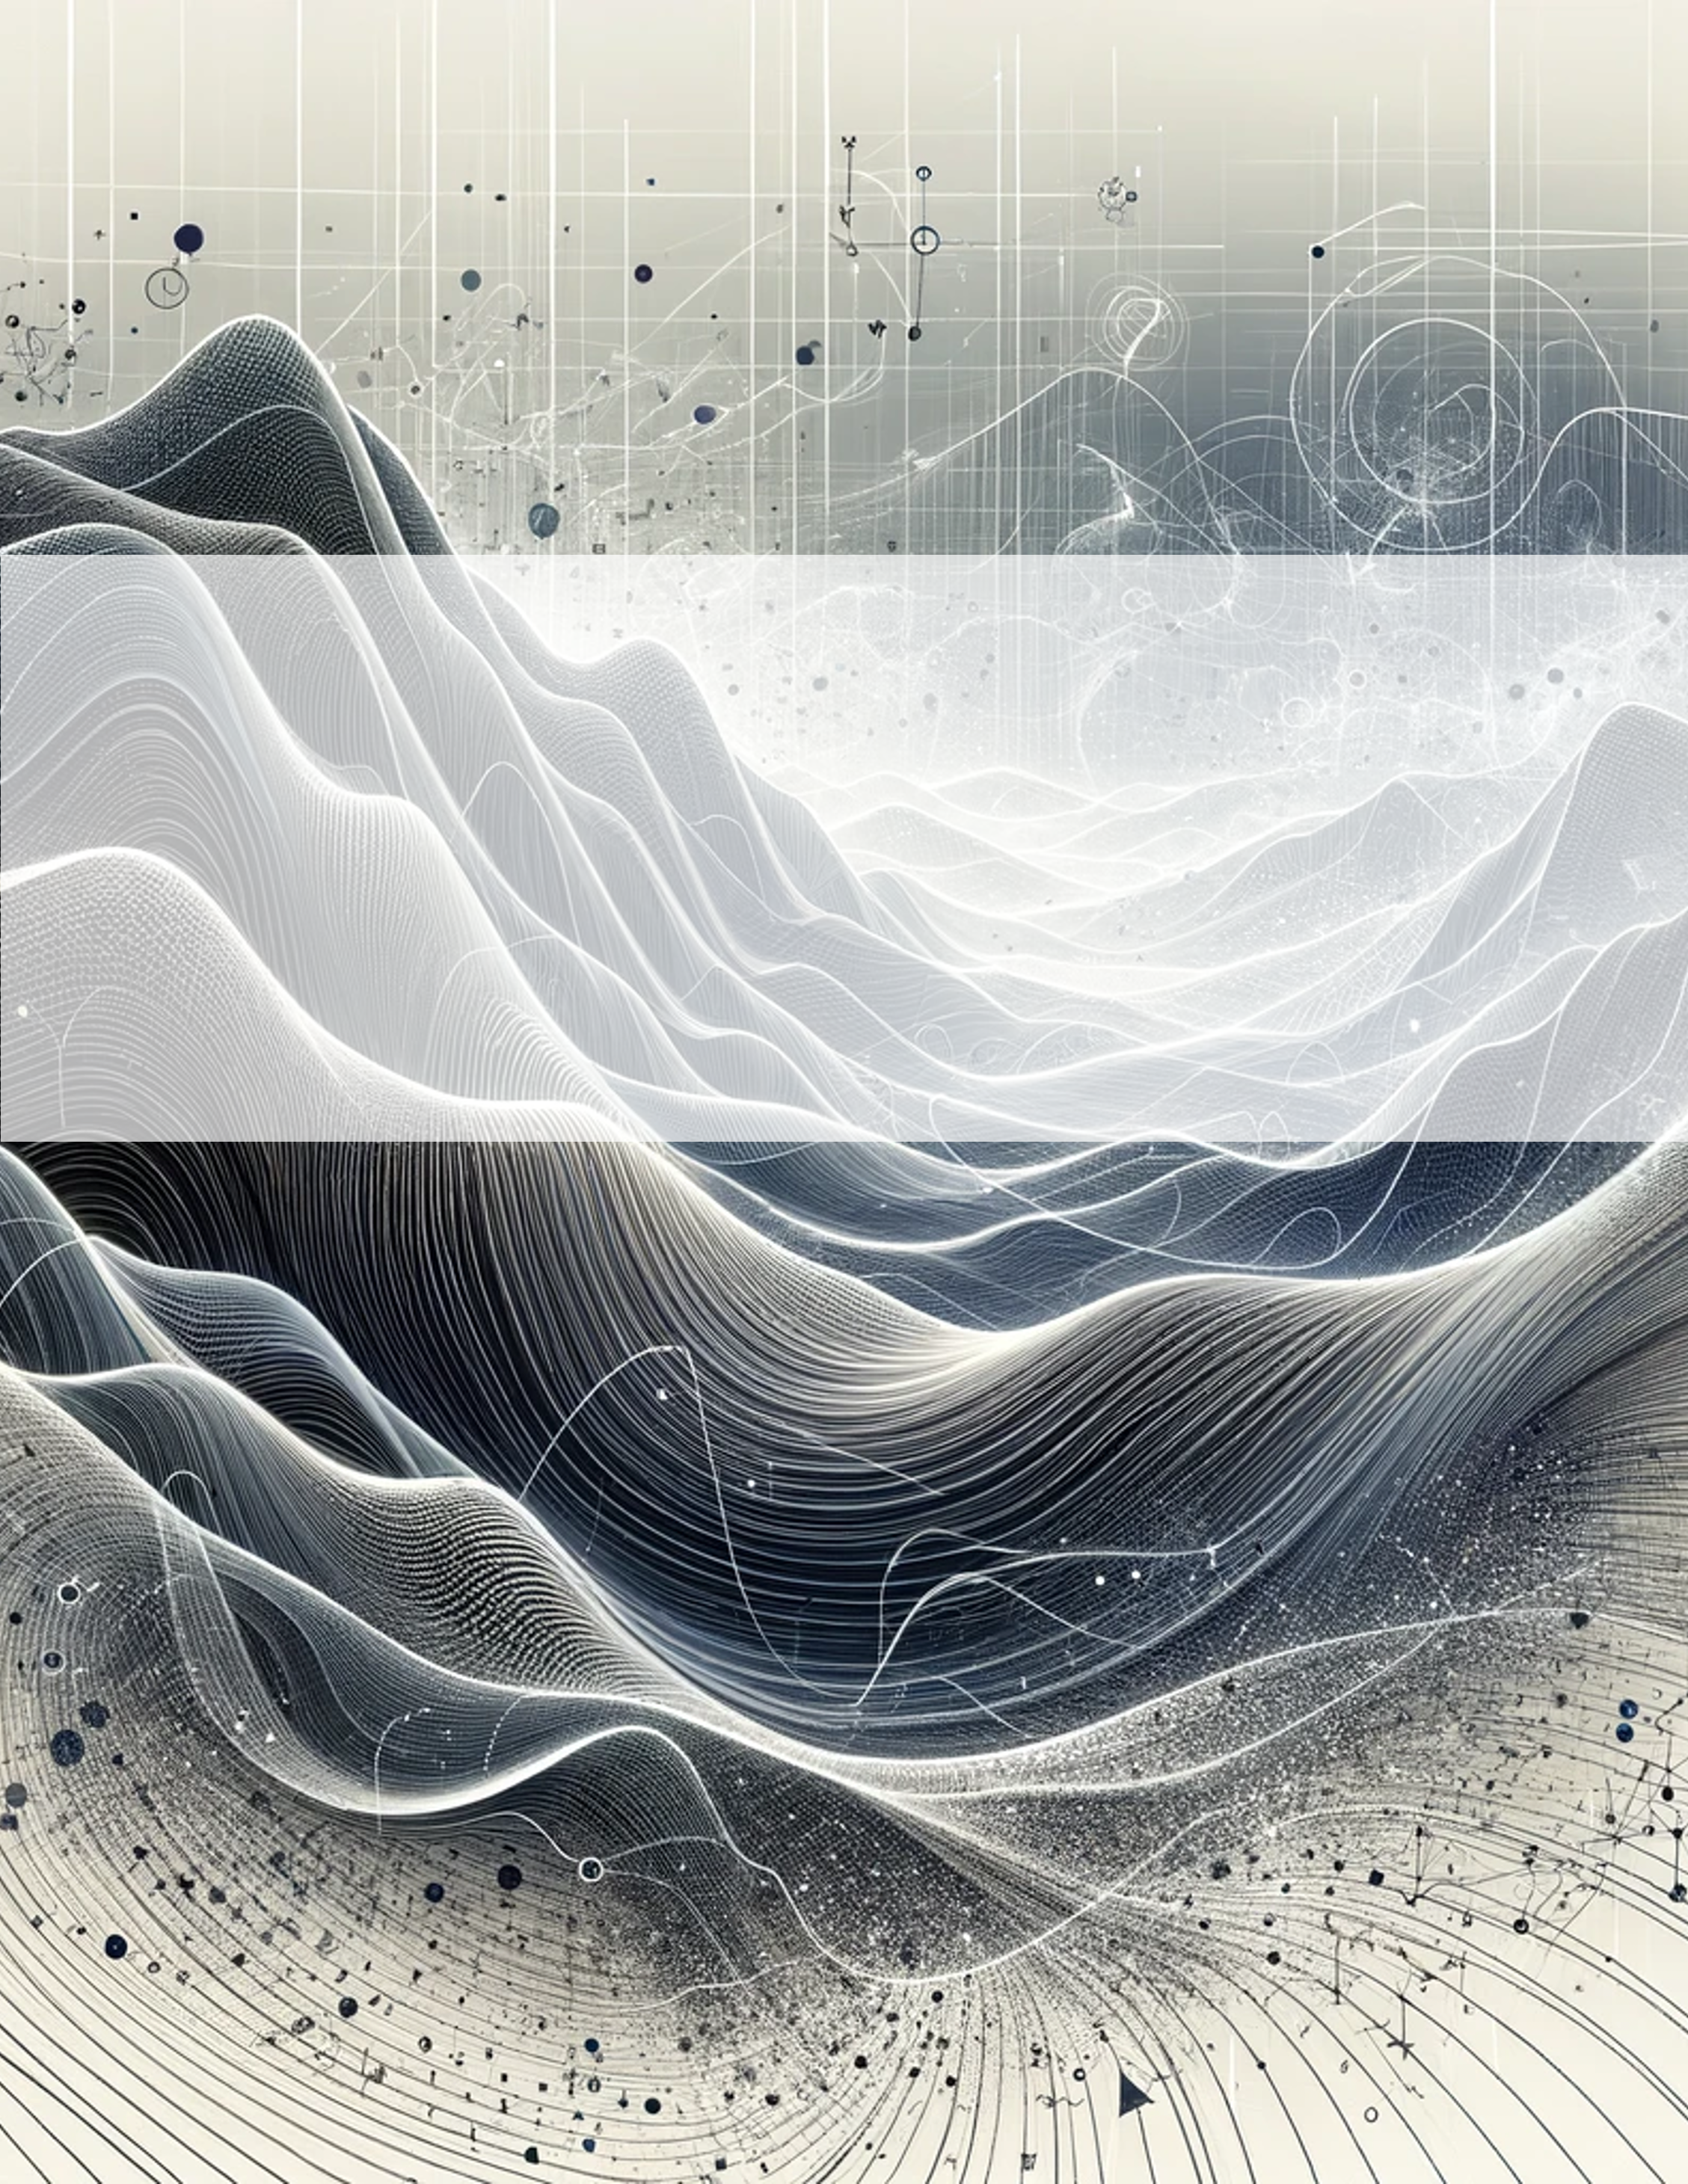
\includegraphics[scale=1.25]{Pictures/bg_title.png}}} % Image background
% \centering
% \vspace*{5cm}
% \par\normalfont\fontsize{35}{35}\sffamily\selectfont
% \textbf{CPSC 542F WINTER 2017}\\
% {\LARGE Convex Analysis and Optimization}\par % Book title
% \vspace*{1cm}
% {\Huge Lecture Notes}\par % Author name
% \endgroup


%----------------------------------------------------------------------------------------
%	TITLE PAGE
%----------------------------------------------------------------------------------------

\begingroup
\thispagestyle{empty}
\AddToShipoutPicture*{\put(0,0){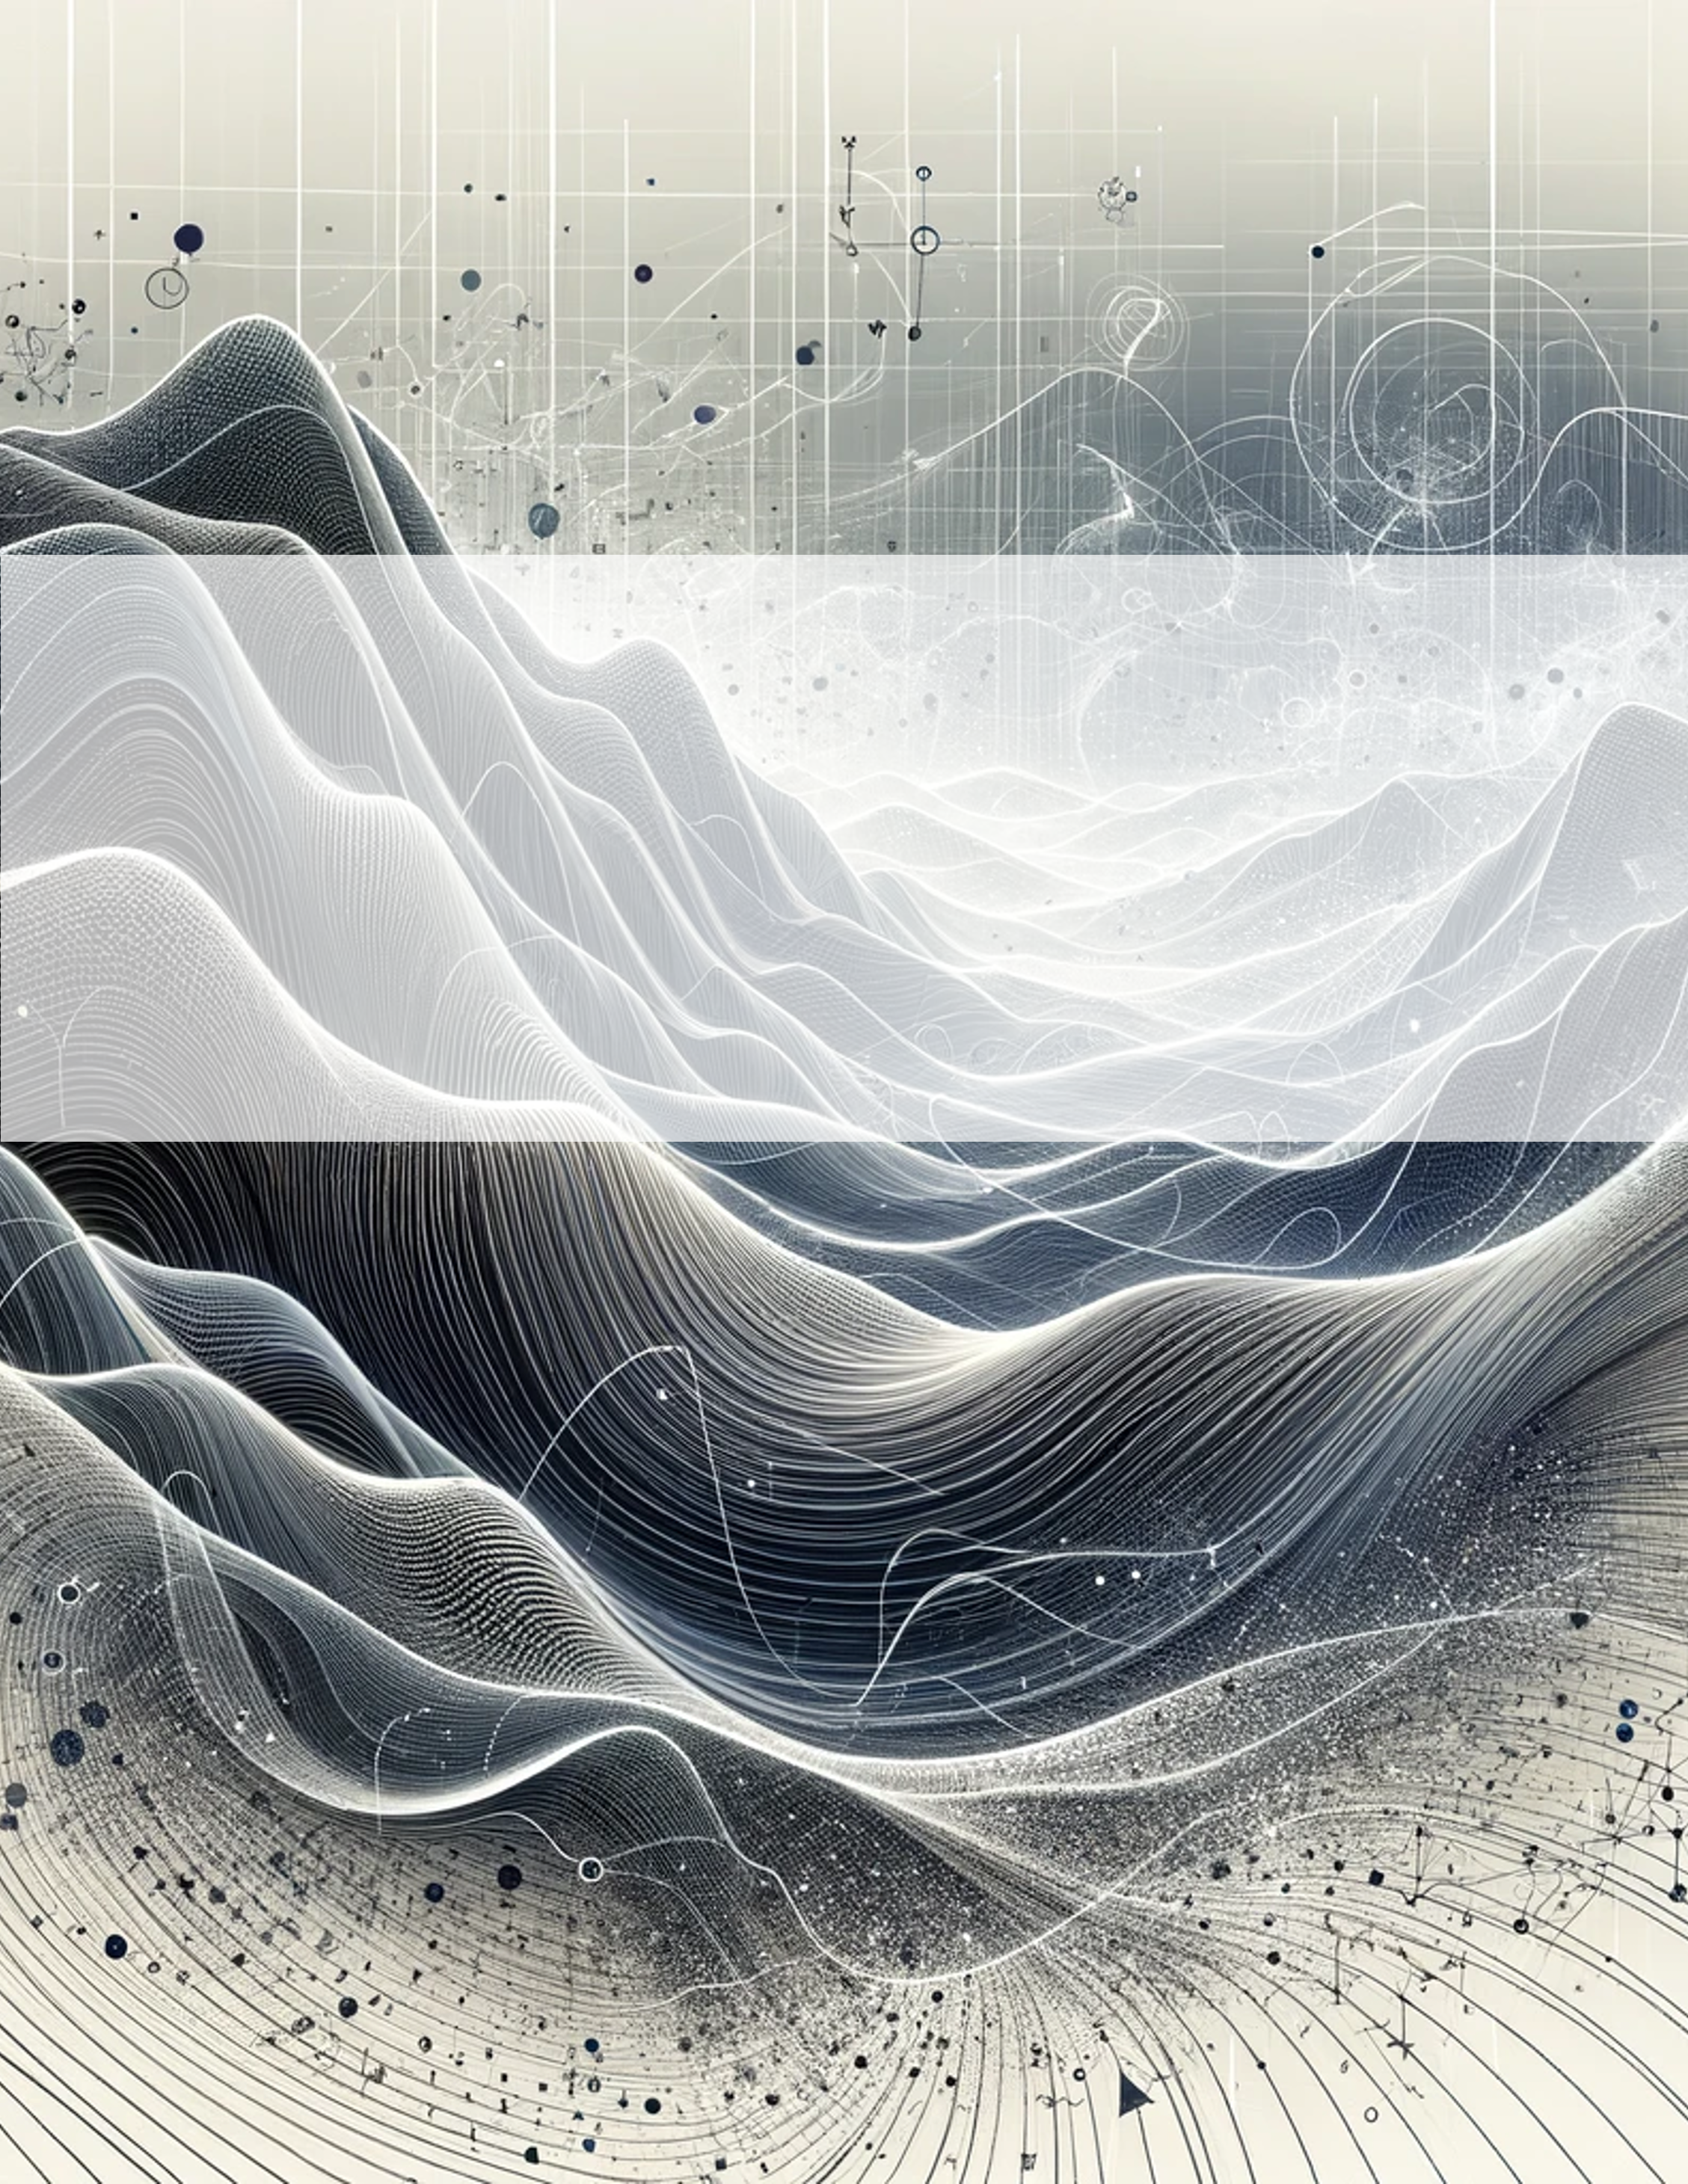
\includegraphics[scale=1.25]{./Pictures/bg_title.png}}} % Image background
\centering
\vspace*{5cm}
\par\normalfont\fontsize{35}{35}\sffamily\selectfont
\textbf{ADA 24A}\\
{\LARGE Análisis y Diseño de Algoritmos}\par % Book title
\vspace*{1cm}
{\Huge Notas de Clase}\par % Author name
\endgroup

%----------------------------------------------------------------------------------------
%	COPYRIGHT PAGE
%----------------------------------------------------------------------------------------

\newpage
~\vfill
\thispagestyle{empty}


\noindent \textsc{Ingeniería en Sistemas y Computación, Universidad de Caldas, Manizales}\\

\noindent \textsc{github.com/OverCV}\\ % URL GitHub

\noindent Estas notas de clase han sido realizadas bajo instrucción de la Dr. Luz Guerrero dentro un total de 16 semanas, desde febrero 05 hasta junio 21 del 2024.\\ % License information

\noindent \textit{Primera publicación, Agosto 2024} % Printing/edition date

%----------------------------------------------------------------------------------------
%	TABLE OF CONTENTS
%----------------------------------------------------------------------------------------

\chapterimage{./Pictures/galaxy.png} % Table of contents heading image

\pagestyle{empty} % No headers
\tableofcontents % Print the table of contents itself

%\cleardoublepage % Forces the first chapter to start on an odd page so it's on the right

\pagestyle{fancy} % Print headers again

%----------------------------------------------------------------------------------------
%	CHAPTER 1
%----------------------------------------------------------------------------------------
\chapterimage{./Pictures/asymptotic_notation.png}
\chapter{Notación asintótica}

Son comprendidas como familias, nos preguntamos si una función particular que pertenece a una familia $X(f(n))$ también pertenece a otra familia $Y(g(n))$. Es así que generamos comparaciones entre funciones.
\section{Crecimiento en funciones}
\subsubsection{Funciones no negativas}
Una $f(x)$ es asintóticamente no negativa si $\exists n_0\in N$ $f(n)$ y se cumpla $(n\ge n_0)\land f(n)\ge0$
Apreciable con la función $f(x)=a~e^{-bx}+cx~e^{-dx}$.

Por definición trabajamos funciones asintóticamente positivas \textit{($t\ge0$)}.

\subsection{Notación Tilde}
$$
	f(n)\sim g(n)\iff\lim_{n\to\infty}\frac{f(n)}{g(n)}=1\implies f(n)\in O(g(n))
$$
Donde convergir a 1 no necesariamente implica sean la misma función.t

\subsection{Big $O$}
\begin{definition}$$
		O(g(n))
		=\{
		f: \mathbb N\to \mathbb R^*~|~(\exists c\in \mathbb R^+)
		(\exists n_0\in \mathbb N)
		(\forall n\ge n_0)
		(0\le f(n)\le c~g(n))
		\}
	$$
	$$
		\lim_{n\to\infty}\frac{f(n)}{g(n)}\leq c
	$$$$
		f(n)=O(g(n))\equiv f(n)\in O(g(n))
	$$
\end{definition}
\begin{remark}Dicción en 'Big Oh':\\
	'Está $f$ acotada superiormente por $g$', 'Es $g$ cota superior a $f$.'
\end{remark}

Si dado $\lim_{n\to\infty}\frac{g(n)}{f(n)}\implies\{\infty: g~\text{crece} > f,~k:g~\text{crece} \approx f,\}$

Si el conjunto de datos está limitado, una función $n^3$ puede ser mejor a una $n^2$.

\begin{example}
	Demostración que $an+b=O(n)$

	Ha de satisfacerse que $an+b\le cn$
	$$
		an+b\le cn      $$$$
		a+\frac bn\le c
	$$
	Es así que tenemos el valor de nuestra constante, podemos apreciar cómo se empezará a cumplir cuando determinemos un valor para $n$ renombrado a $n_0$, desde ese punto se cumplirá la notación.
\end{example}


\subsection{Big $\Omega$}
\begin{definition}$$
		\Omega(g(n)) =\{ f: \mathbb N \to \mathbb R^*  | (\exists c\in \mathbb R^+) (\exists n_0\in \mathbb N) (\forall n\ge n_0) ( 0\le cg(n) \le   f(n) ) \}
	$$$$
		c\le\lim_{n\to\infty}\frac{f(n)}{g(n)}
	$$\end{definition}


\begin{remark}Dicción en 'Big Omega':

	'Está $f$ acotada asintóticamente por debajo por $g$', 'Es $g$ una cota inferior asintótica para $f$'.
\end{remark}


\subsection{Big $\Theta$}
\begin{definition}
	$$
		\Theta   (g(n)) =\{ f : \mathbb N \to \mathbb R^* | (\exists c_1, c_2 \in \mathbb R^+) ( \exists n_0\in \mathbb N) (\forall n \ge n_0) (0\le c_1 g(n) \le f(n) \le c_2 g(n)) \}
	$$$$
		c_1\le\lim_{n\to\infty}\frac{f(n)}{g(n)}\le c_2
	$$\end{definition}

\begin{remark}Dicción en 'Big Theta':

	'Está $f$ acotada estrechamente por $g$', 'Es $g$ una cota estrecha para $f$'.
\end{remark}
Cada miembro de $\Theta(g(n))$ es asintóticamente no negativo así como la función misma \textit{(si no $\Theta{g(n)}=\emptyset$)}

\begin{theorem}
	$\Theta(f(n)) =O(f(n))\cap \Omega(f(n))$
\end{theorem}

\subsubsection{Propiedades}
Un algoritmo $\alpha$ clasifica sí y solo si tiene
\begin{itemize}
	\item Peor tiempo de ejecución es $O(f(n)).$
	\item Mejor tiempo de ejecución es $\Omega(f(n)).$
\end{itemize}

\begin{example}
	Demostración que $0.5n^2-3n=\Theta(n^2)$

	Ha de satisfacerse que $c_1n^2\le 0.5n^2-3n\le c_2n^2$
	$$
		c_1n^2\le 0.5n^2-3n\le c_2n^2
	$$$$
		c_1\le 0.5-3/n\le c_2
	$$
	La inecuación derecha se mantiene para $n\ge1$ si tomamos $c_2\ge0.5$. La inecuación izquierda con $n\ge7$ y escogiendo $c_1<1/14$.
\end{example}

\subsection{Little $o$}
\begin{definition}
	$$
		o (g(n)) = \{ f : \mathbb N \to \mathbb R^* | (\forall c \in \mathbb R^+) (\exists n_0\in \mathbb N) (\forall n\ge n_0) ( 0 \le  f(n) < cg (n) ) \}
	$$$$
		\lim_{n\to\infty}\frac{f(n)}{g(n)} = 0;\quad
		\lim_{n\to\infty}\frac{g(n)}{f(n)}= \infty
	$$
\end{definition}
Son las funciones $o(g(n))$ que crecen más lento que $g$.
\begin{remark}Dicción en 'Little oh':

	'$f$ es asintóticamente más pequeña a $g$'. '$g$ es cota \textit{estríctamente débil} superior a $f$'
\end{remark}

\begin{proof}
	Es $n=o(n^2)$

	Ha de satisfacerse que: $$
		\lim_{n\to\infty}\frac n{n^2}=\lim_{n\to\infty}\frac 1{n}=0
	$$
\end{proof}
\begin{proof}
	Es $n\neq o(3n)$

	Ha de satisfacerse que: $$
		\lim_{n\to\infty}\frac n{3n}=\lim_{n\to\infty}\frac 13=\frac 13\neq0
	$$
\end{proof}

\subsection{Little $\omega$}
\begin{definition}
	$$
		\omega (g(n)) = \{ f : \mathbb N \to \mathbb R^* | (\forall c\in \mathbb R^+) (\exists n_0\in \mathbb N) (\forall n\ge n_0) ( 0 \le  c g(n) < f(n) ) \}
	$$$$
		\lim_{n\to\infty}\frac{f(n)}{g(n)}= \infty;\quad
		\lim_{n\to\infty}\frac{g(n)}{f(n)}= 0
	$$
\end{definition}
Las funciones $\omega({g(n)})$ crecen más rápido que $g$.
\begin{remark}Dicción en 'Little omega':

	'$f$ es asintóticamente más grande a $g$'. '$g$ es cota débil inferior a $f$'.
\end{remark}

\begin{theorem}[Análogo entre números $\mathbb{R}$ y Notación asintótica]
	% Existe esta fácil re-interpretación de lo expuesto.
	$$\begin{array}{cc}
			\text{\textbf{Notación asintótica}} & \text{\textbf{Número real}} \\
			f(n) \in O(g(n))                    & f\le g                      \\
			f(n) \in \Omega(g(n))               & f\ge g                      \\
			f(n) \in \Theta(g(n))               & f= g                        \\
			f(n) \in o(g(n))                    & f< g                        \\
			f(n) \in \omega(g(n))               & f> g                        \\
		\end{array}$$
	\textit{No se mantiene la tricotomía.}
\end{theorem}

\begin{remark}
	\textit{\textbf{Notación Little;} No son asintóticamente estrechas.}
\end{remark}

% \subsubsection{Ejercicios}
% Practicar relaciones con
% \begin{itemize}
%     \item A: $5n^2+100n$, B: $3n^2+2$;    $A\in X(B)$
%     \item A: $\log_3n^2$, B: $\log_2n^3$; $A\in X(B)$
%     \item A: $n^{\lg4}$,  B: $3^{\lg n}$; $A\in X(B)$
%     \item A: $\lg^2n$,    B: $n^\frac12$; $A\in X(B)$
% \end{itemize}

\subsection{Propiedades generales}
\subsubsection{Transitividad}
$$
	(f(n)\in\Delta[g(n)] \land g(n)\in\Delta[h(n)])
	\implies
	(f(n)\in\Delta[h(n)]) $$ $$
	\forall\Delta=O,~\Omega,~\Theta
$$
\subsubsection{Reflexividad}
$$
	f(n)\in\Delta[f(n)] $$ $$
	\forall\Delta=O,~\Omega,~\Theta
$$
\subsubsection{Simetría}
$$
	f(n)\in\Theta(g(n))
	\iff
	g(n)\in\Theta(f(n))
$$ $$
	\forall\Theta
$$
\subsubsection{Anti simetría}
$$
	\forall f(n)\not\in \Theta(g(n))
$$ $$
	f(n)\in\Delta[g(n)]
	\implies
	g(n)\not\in\Delta[f(n)] $$ $$
	\forall\Delta= O,~\Omega
$$
\subsubsection{Simetría transpuesta}
$$
	f(n)\in O(g(n))
	\iff
	g(n)\in\Omega(f(n))
$$ $$
	f(n)\in o(g(n))
	\iff
	g(n)\in\omega(f(n)) $$ $$
	\forall\Delta= O,~\Omega
$$
\begin{theorem}[Órdenes de relación]
	$$\begin{array} {|r|r|r|r|r|}
			\hline \text{Órden}                    & \text{Relexiva} & \text{Simétrica} & \text{Anti simétrica} & \text{Transitiva} \\
			\hline f\le g\iff f(n)\in O(g(n))      & \text{Sí}       &                  & \text{Sí}             & \text{Sí}         \\
			\hline f\ge g\iff f(n)\in \Omega(g(n)) & \text{Sí}       &                  & \text{Sí}             & \text{Sí}         \\
			\hline f= g\iff f(n)\in \Theta(g(n))   & \text{Sí}       & \text{Sí}        &                       & \text{Sí}         \\
			\hline
		\end{array}$$

	Con esto se pueden comprender las relaciones como
	\begin{itemize}
		\item Entre $o\land O$
		      $$  f(n)\in o(g(n)) \implies f(n)\in O(g(n))  $$
		\item Entre $\omega\land\Omega$
		      $$  g(n)\in \omega(f(n)) \implies g(n)\in \Omega(f(n))  $$
	\end{itemize}
	Siempre que $o(f(n))\cap \omega(f(n))=\emptyset$.
\end{theorem}

\begin{example}
	Realizemos estos ejercicios
\end{example}

\subsection{A dos variables}
\begin{definition}
	$$O(g(m,n))=\{f:\mathbb N\times \mathbb N\to \mathbb R^*~|~
	$$ $$
		(\exists c\in \mathbb R^+)
		(\exists  m_0 , n_0 \in \mathbb N)
		(\forall  n\ge  n_0)
		(\forall  m\ge  m_0)
		(f(m, n) \le  c g(m, n))
		\}
	$$
\end{definition}

\begin{example}[Ejercicio]
	Del 1, 2 demostrar si V o F.
	\begin{enumerate}
		\item Para cualquier función $f$ se tiene que $f\in O(f)$. \textit{[V].}
		\item $O(f)=O(g)\iff f\in O(g)\land g\in O(f)$. \textit{[V].}
		\item Para cuáles notaciones es válido afirmar; $f\in \Delta[g]\land g\in\Delta[h]\implies f\in\Delta[h]$
		\item Si $\lim_{n\to\infty}\frac{f(n)}{g(n)}=k$ dependiendo de los valores en $k$.
		      \begin{enumerate}
			      \item Si $k=0\land k<0\implies O(f)=O(g)$
			      \item Si $k\neq0\land k<0\implies O(f)\in O(g)$
		      \end{enumerate}
	\end{enumerate}
\end{example}





\section{Funciones comúnes}
\subsection{Monótomamente incremental}
\begin{definition}
	$$\forall m\le   n \implies f(m)\le  f(n)$$
\end{definition}

\begin{definition}[Función suelo]
	El $\lfloor x\rfloor=\max(\mathbb{Z})\le x$
\end{definition}
\begin{definition}[Función techo]
	El $\lceil x\rceil=\min(\mathbb{Z})\ge x$
\end{definition}
$$
	\forall x\in\mathbb{R},\quad x-1<\floor{x}\le x\le \ceil{x}<x+1
$$ $$
	\forall x\in\mathbb{N},\quad (\floor{x}=x= \ceil{x})\land (\floor{x/2}+\ceil{x/2}=x)
$$
\begin{theorem}
	$$\forall x\in\mathbb R \land \mathbb Z:a,~b>0 $$
	$$ \floor{\frac{\floor{x/a}}b}=\floor{\frac x{ab}} $$
	$$ \ceil{\frac{\ceil{x/a}}b}=\ceil{\frac x{ab}} $$
	$$ \floor{a/b}\le (a+(b-1))/b $$
	$$ \ceil{a/b}\le (a-(b-1))/b $$
	Cabe mencionar estas funciones son monótomamente incrementales.
\end{theorem}

\begin{definition}[Función exponencial]
	Si $\forall n: a\ge0\implies a^n$ es monótomamente incremental.

	Si $\forall(a,b) \in \mathbb R,\quad a>1$ y
	$$ \lim_{n\to\infty}\frac{n^d}{a^n}=0 \implies n^d=o(a^n)$$
\end{definition}

\subsection{Monótomamente decremental}
\begin{definition}
	$$\forall 	 m\le   n \implies  f(m)\ge  f(n)$$
\end{definition}
\subsection{Estríctamente incremental}
\begin{definition}
	$$\forall 	 m<   n \implies  f(m)<  f(n)$$
\end{definition}
\subsection{Estríctamente decremental}
\begin{definition}
	$$\forall 	 m<   n \implies  f(m)>  f(n)$$
\end{definition}

\subsection{Aritmética modular}
\begin{theorem}
	$$\forall \mathbb Z a \land \exists\mathbb Z^+ n$$
	$$ a\mod{n}=a-n\floor{a/n}$$
	El residuo del cociente $\frac an$
\end{theorem}
\begin{theorem}[Equivalencias]
	Si $a\mod n = b\mod n\implies a\equiv b \mod n$
	dictamos $a$ es congruente o equivalente con $b\mod n$. Dan el mismo residuo al dividirse por $n$. Lo será sí y sólo si $n$ es divisor de $b-a$
\end{theorem}

\subsection{Polinomios}
Son funciones de la forma;
$$
	p(n)=\sum_{i=0}^d a_in^i.\quad d>0
$$
Con coeficientes $a_0,a_1, \cdots,a_d\land a_d\neq0$
\begin{theorem}~
	\begin{itemize}
		\item Es $p(n)$ asintóticamente positivo sí y sólo si $a_d>0$.
		\item Sea $p(n)$ de grado $d$ asintóticamente positivo entonces $p(n)=\Theta(n^d)$.
		\item $\forall a\in \mathbb R,\quad a\ge0,\quad n^a$ es monótomamente incremental.
		\item $\forall a\in \mathbb R,\quad a\le0,\quad n^a$ es monótomamente decremental.
		\item $f(n)$ es polinómicamente acotada si $f(n)=O(n^d)$ para algúna constante $d$.
	\end{itemize}
\end{theorem}

\subsection{Logaritmos}
\begin{definition}[Notaciones]
	$$\lg n\equiv \log_2 n$$
	$$\ln n\equiv \log_e n$$
	$$\lg^k n\equiv (\lg n)^k$$
	$$\lg\lg n\equiv \lg(\lg n)$$
	Sólo aplican sobre el siguiente término.
	$$ \lg n+k\equiv (\lg n) +k $$
	Es incremental para $b>1\land n>0$
\end{definition}


\begin{theorem}[Identidades]
	Para los reales $(a,b,c>0)\land n$ tenemos las siguientes identidades
	\begin{enumerate}
		\item $a=b^{\log_ba}$
		\item $\log_c(ab)=\log_ca+\log_cb$
		\item $\log_ba^n=n\log_ba$
		\item $\log_ba=\frac{\log_ca}{\log_cb}$
		\item $\log_ba=1/\log_ab$
		\item $a^{\log_bc}=c^{\log_ba}$
	\end{enumerate}
\end{theorem}

\subsection{Factoriales}
\begin{definition}~

	Sin recursión:
	$$n!=
		\begin{cases}
			n=0\implies 1 \\
			n>0\implies \prod_{i=1}^n i
		\end{cases}$$
	Con recursión:
	$$n!=
		\begin{cases}
			n=0 \implies 1 \\
			n>0 \implies n(n-1)!
		\end{cases}$$
\end{definition}

\begin{fact}
	Cota débil superior:
	$$n!\le n^n$$
\end{fact}

Re-expresiones del factorial:
$$ (n+1)!=n!(n+1) $$
$$ n! =  $$

\subsection{Iteración funcional}
Dada $f(n)$, la i-th iteración funcional es:
$$f^{(i)}:
	\begin{cases}
		i=0\implies I \\
		i>0\implies f(f^{(i-1)})
	\end{cases}$$
Sea $I$ la función identidad, con $n$ particular:
$$f^{(i)}(n):
	\begin{cases}
		i=0\implies n \\
		i>0\implies f(f^{(i-1)}(n))
	\end{cases}$$

\subsection{Logaritmo estrella}
\begin{definition}
	$\lg^*n=\min\{i\ge0~|~\lg^{i}n\le1\}$

	Elevando $k$ veces:
	$$ \lg^*2^{2^{\cdots^{2}}}=k $$
\end{definition}
\begin{fact}[Crecimiento]
	$$ \lg^*2^0=0 $$
	$$ \lg^*2^1=1 $$
	$$ \lg^*2^2=2 $$
	$$ \lg^*2^4=3 $$
	$$ \lg^*2^{16}=4 $$
	$$ \lg^*2^{256}=5 $$
	$$ \vdots $$
	Su crecimiento es ínfimo.
\end{fact}


%----------------------------------------------------------------------------------------
%	CHAPTER 2
%----------------------------------------------------------------------------------------
\chapterimage{./Pictures/algorithmic_analysis.png} % Chapter heading image


%----------------------------------------------------------------------------------------
%   CHAPTER 2
%----------------------------------------------------------------------------------------
\chapterimage{./Pictures/algorithmic_analysis.png}
\chapter{Análisis algorítmico}

Estamos acostumbrados a manejar estructuras:
\begin{itemize}
	\item De control: if, else if, else, anidaciones.
	\item De flujo: for, while, repeat.
	\item De secuencia: Donde las instrucciones (accion $i$) se ejecutan sucesivamente sin omisiones (accion $i$ requiere accion $i-1$).
\end{itemize}

\section{Introducción}
Un algoritmo es el conjunto de procedimientos o funciones o bloques con estructuras de control, deben ser precisos y dar término.
Una función $func$ realizan una tarea y devuelven un valor como resultado o salida.
Un procedimiento $proc$ es un fragmento de código que no retorna un dato sino que trabaja mutando los datos del encabezado.
Los parámetros de un algoritmo son 03:
\begin{enumerate}
	\item Forma: Entrada, Salida o Mixta.
	\item Tipo: La estructura o tipo de dato.
	\item Nombre: Clave cual referencia la variable.
\end{enumerate}
% \newpage
\begin{example}[Costeo algorítmico]~
	\\

	Dado el procedimiento $P0$ en cada línea debemos costear: Número de operaciones elementales, Número de ejecuciones.
	\begin{multicols}{2}
		\begin{lstlisting}
1| proc P0(E int n):
2|     x = 100
3|     z = x + 5
4|     for (i = 1 to n) do
5|         for (j = 1 to n) do
6|             x = x + 1
        \end{lstlisting}
		\columnbreak
		\begin{enumerate}
			\item Llamado sin coste asociado.
			\item $1\times1$
			\item $2\times1$
			\item $3\times\sum_{i=1}^{n+1}1$
			\item $3\times\sum_{i=1}^{n}\sum_{j=1}^{n+1}1$
			\item $2\times\sum_{i=1}^{n}\sum_{j=1}^{n}1$
		\end{enumerate}
	\end{multicols}
	En este escenario al usarse un for se iterará siempre la misma cantidad, con ello estamos en un caso invariante o promedio.
	\\Nótese como siempre el número de ejecuciones en un ciclo se sigue por: $cabeza=cuerpo+1$.
	Eventualmente resolviendo las sumatorias obtenemos la función de eficiencia para el Coste en Complejidad Computacional Temporal \textit{(CC.T(n))}:
	$$
		T(n)=1\times1+2\times1+3\times(n+1)+3\times n\times(n+1)+2\times n\times n
	$$ $$
		T(n)=an^2+bn+c\in \Theta(n^2)
	$$
	Si realizamos el costeo en términos de la Complejidad Computacional Espacial \textit{(CC.S(n))} notamos como sólo se realizan operaciones elementales, todas con un coste constante $(c)$.
	$$
		S(n)=c\in\Theta(1)
	$$
\end{example}

La jerarquía de operaciones para cálculos computacionales es:
\begin{enumerate}
	\item Brackets.
	\item Powers.
	\item Products, Ratios.
	\item Relational operations.
\end{enumerate}

Realizado sobre una función:
\subsection{Sequential Search}
\begin{example}[Análisis búsqueda secuencial]~
	\\Deben definirse:
	\\\textbf{Precondiciones:} Lo que entra; Un arreglo de números enteros y un número entero.
	\\\textbf{Poscondiciones:} Lo obtenido y cómo se obtiene, además de excepciones; Índice del elemento (número entero) ingresado en el arreglo, si no existe retorna $-1$.

	\begin{multicols}{2}
		\begin{lstlisting}
1| func seq_search(
 |   E list[int] A[n], int x, S int p
 | ):
2|     int i = 1
3|     repeat:
4|         if A(i) == x:
5|             return i
6|         i++
7|     until i > n
8|     return -1
        \end{lstlisting}

		\columnbreak
		El mejor escenario o $T_{best}$ es que exista el elemento y sea el primero en la lista.
		\begin{enumerate}
			\item Sin coste.
			\item $1\times1$
			\item Sin coste.
			\item $1\times1$
			\item $1\times1$
			\item $0\times1$
			\item $0\times1$
			\item $0\times1$
		\end{enumerate}
	\end{multicols}

	$$
		T_{best}(n)=1\times1+1\times1+1\times1
	$$ $$
		T_{best}(n)=c\in O(1)
	$$
	No obstante aún faltan escenarios.
	\begin{multicols}{2}
		\begin{lstlisting}
1| func seq_search(
 |   E list[int] A[n], int x, S int p
 | ):
2|     int i = 1
3|     repeat:
4|         if A(i) == x:
5|             return i
6|         i++
7|     until i > n
8|     return -1
        \end{lstlisting}

		\columnbreak
		El peor escenario o $T_{worst}$ es que no exista el elemento.
		\begin{enumerate}
			\item Sin coste.
			\item $1\times1$
			\item $0\times n$
			\item $1\times n$
			\item $0\times n$
			\item $1\times n$
			\item $1\times n$
			\item $1\times1$
		\end{enumerate}
	\end{multicols}
	$$
		T_{worst}(n)= 1\times1+1\times n+1\times 1\times n+1\times1
	$$ $$
		T_{worst}(n)= an+b\in O(n)
	$$
\end{example}


\section{Probabilidad}
\subsection{Eventos deterministas}
\begin{definition}[Suceso elemental]
	Recoge información de todo el experimento
	\begin{example}[Dados]~
		\\Lanzar un dado genera 1 resultado o suceso elemental; Tras 10 resultados generamos un prorrateo, una razón.
	\end{example}
\end{definition}

\begin{definition}[Sucesos]
	\textbf{Seguro}: Donde la probabilidad del evento es 1, $P(S)=1$.
	\textbf{Imposible}: Donde la probabilidad del evento es 0, $P(S)=0$.
\end{definition}

\subsubsection{Probabilidad condicional}
Definida como $P(S|T)=\frac{P(S\cap T)}{P(T)}$

\begin{example}[Dados]~
	\\Tras lanzar 02 dados se tiene que $(S_1:D_1~\text{cae}~1)$, para $(S_2:D_2~\text{cae}~6)$ y el $(S_3:D_1+D_2\le4$. Se busca hallar la $P(S_1|S_3)$.
	\\Encontramos que $P(S_1)=6/36=1/6$, la $P(S_3)=6/36=1/6$ y que la $P(S_1\cap S_3)=3/36=1/12$.
	$$
		P(S_1|S_3)=\frac{3/36}{6/36}=1/2
	$$
\end{example}

\section{Principio de correctitud}
Un algoritmo es correcto si para cada posible entrada se termina con la salida correcta \textit{(hace lo que afirma hacer)}, hay 02 pruebas.


\begin{itemize}
	\item{Correctitud parcial}:
	      Si el algoritmo no hace \textit{halting} entonces se produce un resultado correcto \textit{(PIM)}.

	\item{Terminación}:
	      Si da término en finitud de pasos, independientemente a la entrada.
\end{itemize}



\subsection{Insertion Sort}
Input: Arreglo  $A = [a_1, \cdots a_n]$.
\\
Process: Indexado lineal e iterandos contiguos, ante $A_j > A_i$ activa subiteración; sobre-escribe valores $A_{j+1} = A_{j}$ para ser decreciente izquierda. Finalmente escribe $x$ en penúltima j-iteración.

\begin{lstlisting}
def insertion_sort(A: list[int | float]) -> list[int | float]:
    ''' Numeric list sorted by insertion '''
    for i in range(1, len(A)):
        x: float = A[i]
        j: int = i-1
        while A[j] > x and j >= 0:
            A[j + 1] = A[j]
            j -= 1
        A[j + 1] = x
    return A
\end{lstlisting}

\subsection{Correctitud}
\begin{definition}[Lazo invariante]
	Sentencia cual prueba la correctitud algorítmica, aplicada sobre variables.
	A demostrar:
	\begin{itemize}
		\item Inicialización: Cierto previo a iteración primera.
		\item Mantenimiento: Si es cierto previo a iteración, permanece cierto previo a próxima.
		\item Terminación: Retorna una propiedad cual muestra la correctitud algorítmica (elemento probatorio).
	\end{itemize}
\end{definition}

\begin{example}[En Insertion sort]
	Tomando $A$ en orden.
	\begin{itemize}
		\item Inicialización: El caso de $A$ tamaño 1 es trivial.
		\item Mantenimiento: Cada elemento es menor a su siguiente.
		\item Terminación: En $i=n+1$ permanecen los elementos originales de $A$ \textbf{ordenados}.
	\end{itemize}
\end{example}

\subsection{Función de eficiencia}

Contar la función más ejecutada \textit{(permite saber el funcionamiento algorítmico)}, es la posible ejecución más anidada.


\begin{example}[Iteraciones múltiples]
	Un ejemplo práctico.

	\begin{lstlisting}
    def triple_for(n: int) -> int:
        x: int = 0
        for i in range(n):
            for j in range(n):
                for k in range(n):
                    x += 1
        return x
    \end{lstlisting}

	Con ello se buscará el comportamiento asintótico más representativo para el código mencionado.
	Para trabajar ciclos es necesaria la representación mediante sumatorias, desde la más interna a la más externa, donde tras resolver el más interno se pasa al más
	externo hasta dejarse como una función de tendencia.

	Supóngase $n=3$ entonces lo primero es contarse cada ejecución en k:
	Haciendo las iteraciones:
	$$triple\_for\begin{cases}
			~i=1:\quad j=(1,2),\quad k=(1,2)          \\
			~i=2:\quad j=(1,2,3),\quad k=(1,2)(1,2,3) \\
			~i=3:\quad j=(1,2,3,4),\quad k=(1,2)(1,2,3)(1,2,3,4)
		\end{cases}$$

	\begin{remark}
		Tenemos en total contando únicamente el número de ejecuciones en $k$, representable por la fórmula:
		$$
			f(n)=\sum_{i=1}^n i^2+i-2 \\
		$$ $$
			=\sum_{i=1}^n i^2 + \sum_{i=1}^n i - \sum_{i=1}^n 2
		$$ $$
			=\frac{n(n+1)(2n+1)}6+\frac{n(n+1)}2-2n
		$$
	\end{remark}
	Es apreciable que tras realizar la distribución de términos $n$ se obtiene $\frac13n^3+\cdots-\frac43n$ como el de mayor grado con otros términos de menor grado. Es así que podemos decir eventualmente tenemos un comportamiento asintótico de $n^3$, expresado \textbf{en la mejor forma} como $\Theta(n^3)$.
\end{example}

\section{Limites}
Tenemos como unos casos especiales que aplican a los límites:
$$
	\lim_{n\to\infty}\br{\frac1n}=0
$$
$$
	\lim_{n\to\infty}\br{\frac n{n+1}}=1
$$
$$
	\lim_{n\to\infty}(\sqrt[n]{a})=0;\quad a>0
$$
$$
	\lim_{n\to\infty}(\sqrt[n]{n})=1
$$
$$
	\lim_{n\to\infty}\br{\frac{ln[n]}{x^n}}=0;\quad(a>0)\land (b>0)
$$
$$
	\lim_{n\to\infty}\br{1+\frac1n}^n=e
$$
$$
	\lim_{n\to\infty}\br{\frac{Sin(x)}x}=1
$$
$$
	\lim_{n\to\infty}ATan(x)=\frac{\pi}2
$$
$$
	\lim_{n\to\infty}ASec(x)=\frac{\pi}2
$$
$$
	\lim_{x\to\infty}f(x)=L
	\implies
	\lim_{n\to\infty}f(n)=L
$$

\section{Series}
Generalización sobre la noción de suma sobre una función $f(n)$ acotada superior e inferiormente.

\subsection{Propiedades}
\begin{theorem}[Adiciones y sustracciones]
	$$
		\sum_{i=0}^n[f(i)\pm g(i)\pm\cdots\pm z(i)]
		= \sum_{i=0}^nf(i)\pm \sum_{i=0}^ng(i)\pm\cdots\pm\sum_{i=0}^nz(i)
	$$
\end{theorem}

\begin{theorem}[Constantes]
	$$ \sum_{i=0}^nc\cdot f(i) = c\cdot\sum_{i=0}^nf(i) $$
\end{theorem}

\begin{theorem}[Cambio de índice]
	$$ \sum_{i=0}^nf(i) = \sum_{i=k}^{n+k}f(i-k) $$
\end{theorem}

\begin{theorem}[Índice a 0]
	$$ \sum_{i=a}^bf(i) = \sum_{i=0}^{b-a}f(i+a) $$
\end{theorem}

\begin{theorem}[Partición]
	$$ \sum_{i=0}^nf(i) = \sum_{i=0}^cf(i)+\sum_{i=c+1}^nf(i) $$
\end{theorem}

\begin{theorem}[Dobles]
	$$
		\sum_{i=0}^p\sum_{j=0}^qf(i,j)
		\equiv \sum_{j=0}^q\sum_{i=0}^pf(i,j)
	$$
\end{theorem}

\subsection{Series comúnes}

\begin{definition}[Aritmética]
	Forma general
	$$ \sum_{i=1}^ni = \frac{n(n+1)}2 $$
	\begin{fact}[Orden]
		$O(n^2)$
	\end{fact}
\end{definition}

\begin{definition}[Geométrica]
	Forma general
	$$ \sum_{i=0}^nar^i = \frac{a(1-r^{n+1})}{1-r}\quad r\ne1 $$
	$a$: Primer término. $r$: Razón común.
	\begin{fact}[Orden]
		$|r|>1:O(r^n);\quad|r|<1:O(1)$
	\end{fact}
\end{definition}

\begin{definition}[Base 2]
	Forma general
	$$ \sum_{i=0}^nar^i = \frac{a(1-r^{n+1})}{1-r};\quad r\ne1 $$
	$a$: Primer término. $r$: Razón común.
	\begin{fact}[Orden]
		$|r|>1:O(r^n);\quad|r|<1:O(1)$
	\end{fact}
\end{definition}

\begin{definition}[Potencias]
	Forma general
	$$ \sum_{i=1}^ni^k$$
	Solución indefinida;
	\begin{remark}Generalización alterna $k=1$:
		$$\sum_{i=0}^nai+b=\frac{(an+2b)(n+1)}2$$
	\end{remark}
	$$
		k=2\implies\frac{2n^3+3n^2+n}6;\quad
		k=3\implies\frac{n^4+2n^3+n^2}4;\quad
	$$ $$
		k=4\implies\frac{6n^5+15n^4+10n^3-n}{30};\quad
		k=5\implies\frac{2n^6+6n^5+5n^4-n^2}{12};
	$$ $$
		k=6\implies\frac{6n^7+21n^6+21n^5-7n^3+n}{42};
	$$ $$
		k=7\implies\frac{3n^8+12n^7+14n^6-7n^4+2n^2}{24};
	$$ $$
		k=8\implies\frac{10n^9+45n^8+60n^7-42n^5+20n^3-3n}{90};
	$$ $$
		k=9\implies\frac{2n^{10}+10n^9+15n^8-14n^6+10n^4-3n^2}{20};
	$$ $$
		k=10\implies\frac{6n^{11}+33n^{10}+55n^9-66n^7+66n^5-33n^3+5n}{66}\dots
	$$

	\begin{fact}[Orden]
		$O(n^{k+1})$
	\end{fact}
\end{definition}

\begin{definition}[Armónica]
	Forma general
	$$ \sum_{i=1}^n\frac1i$$
	Solución indefinida;
	$$ \ln n+\gamma.\quad\gamma:\text{Euler-Mascheroni}=-\int_0^\infty e^{-x}\ln x~dx $$
	\begin{fact}[Orden]
		$O(\ln n)$
	\end{fact}
\end{definition}


\begin{definition}[Logarítmica]
	Forma general
	$$ \sum_{i=1}^n\log i \approx
		n\log n-n$$
	\begin{fact}[Orden]
		$O(n\log n)$
	\end{fact}
\end{definition}

\subsection{Productorias}

\begin{definition}[Factorial]
	$$
		\prod_{i=1}^ni
		=n!
	$$
\end{definition}

\begin{definition}[Constante]
	$$
		\prod_{i=1}^nk
		=k^n
	$$
\end{definition}

\begin{definition}[Generalizada]
	$$
		\prod_{i}^n a_{i+1}
		=k^n\prod_{i=1}^ni
	$$
\end{definition}

\begin{definition}[Escalar]
	$$
		\prod_{i=1}^nki
		=k^n\prod_{i=1}^ni
	$$
\end{definition}

\subsubsection{Propiedades telescópicas}

\begin{definition}[Generalizada]
	$$
		\prod_{i}^n a_{i+1}
		=k^n\prod_{i=1}^ni
	$$
\end{definition}

\subsubsection{Correlación}
\begin{definition}
	$$
		\lg \prod_{i=1}^n a_i
		= \sum_{i=1}^n\lg a_i
	$$
	$$
		\prod_{i=1}^n a_i
		= 2^{\sum_{i=1}^n\lg a_i}
	$$
\end{definition}

\subsection{Límites}
Es fundamental conocer los límites de cualquier función matemática para establecer relaciones próximamente en notaciones asintóticas. Recordemos sus propiedades:

$$\begin{array} {|r|r|}
		\hline  \text{Constantes}
		 & \quad\lim_{x\to c}k
		=k    \quad                                        \\
		\hline  \text{Identidad}
		 & \quad\lim_{x\to c}x
		=c    \quad                                        \\
		\hline  \text{Escalar}
		 & \quad\lim_{x\to c}kf(x)
		=k\lim_{x\to c}f(x)    \quad                       \\
		\hline  \text{Exponente}
		 & \quad\lim_{x\to c}x^p
		=c^p;    \quad r\ge0\quad                          \\
		\hline  \text{Adición}
		 & \quad\lim_{x\to c}[f(x)+g(x)]
		=\lim_{x\to c}f(x)+\lim_{x\to c}g(x)    \quad      \\
		\hline  \text{Substracción}
		 & \quad\lim_{x\to c}[f(x)-g(x)]
		=\lim_{x\to c}f(x)-\lim_{x\to c}g(x)    \quad      \\
		\hline  \text{Producto}
		 & \quad\lim_{x\to c}[f(x)\times g(x)]
		=\lim_{x\to c}f(x)\times\lim_{x\to c}g(x)    \quad \\
		\hline  \text{Razón}
		 & \quad\lim_{x\to c}[f(x)\div g(x)]
		=\lim_{x\to c}f(x)\div\lim_{x\to c}g(x);
		\quad \lim_{x\to c}g(x)\ne0                        \\
		\hline  \text{Potencia}
		 & \quad\lim_{x\to c}f(x)^{g(x)}
		=\lim_{x\to c}f(x)^{\lim_{x\to c}g(x)};
		\quad f(x)>0                                       \\
		\hline  \text{Logaritmo}
		 & \quad\lim_{x\to c}[\log f(x)]
		=\log[\lim_{x\to c}f(x)]    \quad                  \\
		\hline  \text{Radical}
		 & \quad\lim_{x\to c}[\sqrt{f(x)}]
		=\sqrt{\lim_{x\to c}f(x)}    \quad                 \\
		\hline
	\end{array}$$

Supóngase que se tiene una sucesión tal que tras hallar su \textit{n-ésimo} término $\lim_{n\to\infty}=L$

Los casos especiales son los siguientes:

$$
	\lim_{n\to\infty}\br{\frac1n}=0
$$ $$
	\lim_{n\to\infty}\br{\frac n{n+1}}=1
$$ $$
	\lim_{n\to\infty}(\sqrt[n]{a})=0;\quad a>0
$$ $$
	\lim_{n\to\infty}(\sqrt[n]n)=1;\quad n>0
$$ $$
	\lim_{n\to\infty}\br{\frac{ln[n]}{x^n}}=0;\quad a,b>0
$$ $$
	\lim_{n\to\infty}\br{1+\frac1n}^n=e;
$$ $$
	\lim_{n\to\infty}\br{\frac{Sin(n)}n}=1
$$ $$
	\lim_{n\to\infty}(ATan(x))=\lim_{n\to\infty}(ASec(x))=\frac{\pi}2
$$

\subsection{Criterios de convergencia}
Es fundamental conocer dada una serie su valor finito convergente.
\subsubsection{Criterio suficiente de divergencia}
Si $\lim_{n\to\infty}a_n$ no existe, o si $\lim_{n\to\infty}a_n\ne0$ entonces la Serie diverge.
~\\
Si el $\lim_{n\to\infty}a_n=0$ entonces \textbf{NO} se concluye nada.
~\\
Si $\sum a_n$ sabemos \textit{converge} entonces $\lim_{n\to\infty}(a_n=0)$.


%----------------------------------------------------------------------------------------
%   CHAPTER 3
%----------------------------------------------------------------------------------------
\chapterimage{./Pictures/divide_n_conquer.png}
\chapter{Divide y vencerás}

\section{Ordenamiento}

\subsection{Merge Sort}

Input: Arreglo A = [$a_0, a_1,\cdots,a_n$]

\begin{definition}[Paradigma]
	\begin{itemize}
		Resolución DyV:
		\item \textbf{Dividir:} Problema $\to$ Sub-problemas $\in type(P_0)$.
		\item \textbf{Conquistar:} $\forall$ Sub-problema (recursiva). size(sub-problema) $\to$ 0.
		\item \textbf{Combinar:} Solución = Sub-problema $+\cdots+$ Sub-problema.
	\end{itemize}
\end{definition}

\begin{example}[En Merge sort]
	\begin{enumerate}
		\item \textbf{Dividir:} A$\to$A[n/2] $\land$ A[n/2].
	\end{enumerate}
\end{example}

Un paso fundamental a realizar es combinar 2 listas ordenadas en sólo una.
\begin{lstlisting}
    def merge(L: list[int], R: list[int]) -> list[int]:
    merged = []
    i: int = 0
    j: int = 0

    while i < len(L) and j < len(R):
        if L[i] <= R[j]:
            merged.append(L[i])
            i += 1
        else:
            merged.append(R[j])
            j += 1

    merged.extend(L[i:])
    merged.extend(R[j:])
    return merged
\end{lstlisting}
La función $merge(...)$ tiene Complejidad computacional temporal \textit{(CC.T)} $T(n)=n$, así como su Complejidad espacial $S(n)=n$ \textit{(Isn't an in-place algorithm)}.
\\\\
El corazón del algoritmo
\begin{lstlisting}
    def merge_sort(A: list[int]) -> list[int]:
    if len(A) == 1:
        return A

    q = len(A) // 2
    L = merge_sort(A[:q])
    R = merge_sort(A[q:])
    return merge(L, R)
\end{lstlisting}
Si la longitud del arreglo $A$ es 1 elemento entonces debemos retornar el mismo puesto es caso base.
Partimos recursivamente el arreglo en 2, tomando su parte derecha e izquierda para mediante retorno \textit{(backtracking)} combinarlos.

\paragraph{Análisis de eficiencia}
Se realizan 02 llamadas dentro el método tal que se realiza una partición del tamaño de la entrada $T(n)=2T(n/2)$, además, en la función $merge(...)$ como se mencionó se hace un consumo lineal de tiempo $n$. Podemos concluír que su función de eficiencia es:
$$ T(n) = 2T(n/2)+n $$

Para cálcular su CC podemos hacer uso de un árbol de recursión, notamos se generan $\lg n$ niveles y en ellos, siempre habrán $n$ elementos \textit{(surgidos de la partición del arreglo)}. Podemos regir entonces cómo el algoritmo $merge\_sort$ maneja una CC.T
$$ merge\_sort:~T(n)\in \Theta(n\lg n) $$

\subsection{Quick sort}
En $quick\_sort(...)$ el principio es escoger un pivote \textit{(preferiblemente random)} sobre el que, si tiene elementos a su izquierda de tamaño inferior o igual y elementos a su derecha de tamaño superior o igual, entonces este pivote está ordenado. Este proceso recursivamente subdivide en 2 listas hasta llegar al caso base \textit{(0 a 1 elemento)} sobre el que se reconstruye la solución.
\begin{lstlisting}
    def quick_sort(A: list[int | float]) -> list[int | float]:
    if len(A) <= 1:
        return A
    pivot: int | float = A[0]
    less: list[int | float] = [x for x in A[1:] if x <= pivot]
    greater: list[int | float] = [y for y in A[1:] if y > pivot]
    return quick_sort(less) + [pivot] + quick_sort(greater)
\end{lstlisting}
Suponiendo el mejor escenario $quick\_sort$ tomará el pivote que corresponda el elemento mediano al arreglo, es así que se puede realizar un Árbol de recursión que tome una altura $\log n$, por cada nivel se tendrán $n$ elementos por lo que así como en $merge\_sort$ su función de eficiencia será $T(n)=n\lg n\in O(n\lg n)$.
\\\\
No obstante en su peor escenario la partición se realiza al inicio de arreglo, con ello se generaría un árbol \textit{(línea)} cual en cada nivel del Árbol de derivación tendrá $n,n-1n\cdots,1$ elementos, con ello su función de eficiencia se denotaría como
$$T(n)=\frac{n(n+1)}2\in O(n^2)$$
Así mismo su análisis de CC.S puede determinarse que haciendo uso de una pila, en el mejor escenario usará un tamaño de $\lg n$ y en el peor uno de $n$. \textit{(El tamaño de la pila depende del tamaño del árbol)}.

El caso medio tenemos:
(El análisis es después que se ejecuta partición)
$$
	T(n)_1=T(0)+T(n-1)+Cn
$$ $$
	T(n)_2=T(1)+T(n-2)+Cn
$$ $$
	T(n)_3=T(2)+T(n-3)+Cn
$$ $$ \vdots $$ $$
	T(n)_{n/2}=T(n/2)+T(n/2)+Cn
$$ $$ \vdots $$ $$
	T(n)_{n-2}=T(n-3)+T(2)+Cn
$$ $$
	T(n)_{n-1}=T(n-2)+T(1)+Cn
$$ $$
	T(n)_n=T(n-1)+T(0)+Cn
$$

Si se supone que tenemos $n$ casos según la posición del pivote.

Entonces podemos formular la siguiente función de eficiencia

$$
	T_{avg}(n)=\sum_{I\in D}T(I)\cdot R(1)
$$
Como notamos es muy distinto a los algoritmos iterativos (acá se miran la cantidad de pasos). Entonces tenemos que calculando la función de eficiencia para todas las posibles entradas de datos camos a ttener una ecuación distinta, sumamos todas las difetentes entradas de datos, por lo que:
$$
	T_A(n)
	=(\frac1n)\sum_{i=1}^n[T(i-1)+T(n-i)]+Cn
$$
Tenemos que $\frac1n$ es la probabilidad de la entrada de datos.

La idea es resolver la ecuación, quedando como:
$$
	T_A(n)=\frac1n(2T(0)+2T(1)+\cdots+2T(n-2)+2T(n-1))+Cn
$$ $$
	T_A(n)=\frac1n(2T(0)+2T(1)+\cdots+2T(n-2)+2T(n-1))+Cn
$$
Es lineal no homogenea.
En Quicksort los el mejor

Iniciamos que no sabemos nada, luego nos paramos en el pivote tras partición, no es que digamos "primera posición", es que dependiendo de cómo hagamos las cosas es que tras elegir lo mejor es que elija el pivote tras ubicarse quede en la mitad y con ello 2 particiones de tamaño n/2 (una cosa es decir el pivote está en $a$, otra es que el pivote queda en $b$), pero, lo peor es que quede en los extremos, donde el pivote genera un arbol desbalanceado

En el mejor escenario de un arreglo $arr=[1,2,3,4,5,6,7]$ es el pivote 4 sería lo mejor que podría pasarme
Pero si escogemos a 1 entonces generamos 2 particiones, una con 0 elementos y otra con n-1

Entonces quien es el pivote? No lo sabemos, no sabemos qué tenemos, nos da lo mismo que sea cualquiera (pero lo mejor), pero el mejor es que toque 4 (ubicadito en la mitad). Si tenemos $[4,2,3,1,5,6,7]$




\subsection{Heaps}
Deben de aclararse la peor escenario, esto s siguientes definciones para comprender un Heap \textit{(montículo)}:

\begin{definition}[Árbol binario pleno]~\\
	Un árbol es pleno si dada una altura $h$ tiene una cantidad de $2^{h+1}-1$ nodos. Cada nivel no tiene espacio para inserción de nodos.
\end{definition}

\begin{definition}[Árbol binario completo]~
	\begin{enumerate}
		\item Si el arreglo representativo no tiene elementos nulos entre elementos existentes.
		\item Si el último nivel tiene sus elementos contiguos de izquierda a derecha \textit{(considerados árboles binarios casi completos)}.
	\end{enumerate}
	Siempre mínimamente la altura será $h=\lg n$ puesto ha de llenar todo el nivel para pasar al otro.
\end{definition}

Entonces podemos definir un Heap como un árbol binario completo.
Un heap cumple las siguientes propiedades:
\begin{itemize}
	\item El elemento \textit{(nodo)} de posición $i$ tiene como nodos hijos a \textit{left} y \textit{right}.

	      Si un nodo está en un índice $i$:
	      \begin{itemize}
		      \item Su hijo $left$ está en $2i$.
		      \item Su hijo $right$ está en $2i+1$.
		      \item Su padre $root$ está en $\floor{i/2}$.
	      \end{itemize}
\end{itemize}~\\
Existen 02 tipos de Heaps; \textbf{Max Heap} y \textbf{Min Heap}.

\subsubsection{Min Heap}
Téngase el arreglo $A_m=[10,30,20,35,40,32,25]$, el nodo posición $i$ es menor o igual a sus hijos; $(A_m[i] \le A_m[2i]) \lor (A_m[i] \le A_m[2i+1])$. Representable como

$$\begin{forest}
		for tree={draw}
		[10
			[30
					[35][40]]
			[20
					[32][25]]
		]
	\end{forest}$$

\subsubsection{Max Heap}
Téngase el arreglo $A_M=[50,30,20,15,10,8,16]$ se aprecia cómo cada padre tiene un valor superior o igual a sus hijos; $(A_M[i] \ge A_M[2i]) \lor (A_M[i] \ge A_M[2i+1])$. Representable como

$$\begin{forest}
		for tree={draw}
		[50
			[30
					[15][10]]
			[20
					[08][16]]
		]
	\end{forest}$$

\begin{theorem}[Añadir $add(x)$]~\\
	Implica dar al elemento $x$ la posición última del arreglo y con ello tener el padre en posición $\floor{i/2}$.
	Adicionalmente para cumplir la propiedad \textbf{Max Heap} debe ordenarse.

	Supóngase buscamos $A.add(60)$, generaría un $A=[50,30,20,15,10,8,16,60]$, si 60 está en posición 8, su $i$ padre es 4 con $A[4]=15$.
	$$\begin{forest}
			for tree={draw}
			[50
				[30
						[15
								[60]]
						[10]]
				[20
						[08][16]]
			]
		\end{forest}$$
	$$
		[i=1:50,i=2:30,i=3:20,i=4:15,i=4:10,i=6:8,i=7:16,i=8:60]
	$$
	Notamos no cumple la propiedad Max Heap, por lo que debemos realizar una serie de cambios entre elementos para volverlo Max Heap.

	Con ello realizamos el cambio $(60\to15)\to(60\to30)\to(60\to50)$, obteniendo
	$$\begin{forest}
			for tree={draw}
			[60
				[50
						[30
								[15]]
						[10]]
				[20
						[08][16]]
			]
		\end{forest}$$
	obtenemos $A=[60,50,20,30,10,8,16,15]$. Este procedimiento puede costarnos entre $O(1)$ a $O(\lg n)$.
\end{theorem}

\begin{theorem}[Optimizado a Heap]~\\
	Existen 02 procesos para optimizar una lista a Heap, mediante \textbf{Create Heap} o la \textbf{Heapify}. La diferencia crucial está en la magnitud de complejidad, mientras Create Heap tiene CC.T $O(n\lg n)$ \textit{($n:$ elementos, $\lg n:$ Asumir se mueven a la raíz)}, mediante Heapify hya CC.T $O(n)$ puesto escanéa cada elemento y si no cumple la propiedad realiza los cambios necesarios.

	\begin{proof}
		Si queremos optimizar (Max/Min Heap) la lista $A=[10,20,15,30,40]$ en $B=[-,-,-,-,-]$ siguiendo el siguiente esquema (representable con árbol):
		\begin{enumerate}
			\item $B=[10,-,-,-,-]$
			\item $B=[10,20,-,-,-]\to[20,10,-,-,-]$
			\item $B=[20,10,15,-,-]$
			\item $B=[20,10,15,30,-]\to[30,20,15,10,-]$
			\item $B=[30,20,15,10,40]\to[40,30,15,10,20]$
		\end{enumerate}
	\end{proof}

	Ahora, si realizamos mediante \textbf{Heapify} tendremos el siguiente esquema:

	\begin{proof}
		Téngase $A=[10,20,15,12,40,25,18]$ representable como heap
		$$\begin{forest}
				for tree={draw}
				[10
					[20
							[12][40]]
					[15
							[25][18]]
				]
			\end{forest}$$
		Para el análisis se hace desde el último a primer $i$, ahora no va de abajo hacia arriba el cambio, si no de arriba a abajo. Verificamos cuáles cumplen la propiedad de Max Heap.

		$$\begin{forest}
				for tree={draw}
				[10
				[20
					[12 $\to$ sat.][40 $\to$ sat.]]
				[15 $\to$ no-sat.
				[25 $\to$ sat.][18 $\to$ sat.]]
				]
			\end{forest}$$
		Claramente las hojas por invariante de inicialización cumplen con la propiedad Max Heap, al llegar a $A[3]=15$ ya no satisface la propiedad, hemos de ordenar.

		Entre sus hijos es $(A[6]>A[7])=(25>18)$, y es $(A[6]\ge A[3])=(25>15)$, queda

		$$\begin{forest}
				for tree={draw}
				[10
				[20 $\to$ no-sat.
				[12 $\to$ sat.][40 $\to$ sat.]]
				[25 $\to$ sat.
					[15 $\to$ sat.][18 $\to$ sat.]]
				]
			\end{forest}$$
		Determinamos $A[5]<A[4]$ por lo que hacemos cambio de $A[2]\land A[5]$, tal que

		$$\begin{forest}
				for tree={draw}
				[10 $\to$ no-sat.
				[40 $\to$ sat.
					[12 $\to$ sat.][20 $\to$ sat.]]
				[25 $\to$ sat.
					[15 $\to$ sat.][18 $\to$ sat.]]
				]
			\end{forest}$$
		Finalmente notamos como $A[1]<A[2]$ y luego $(A[1]\to A[2])<A[5]$ para tener

		$$\begin{forest}
				for tree={draw}
				[40 $\to$ sat.
					[20 $\to$ sat.
							[12 $\to$ sat.][10 $\to$ sat.]]
					[25 $\to$ sat.
							[15 $\to$ sat.][18 $\to$ sat.]]
				]
			\end{forest}$$
		Con $A=[40,20,15,12,10,25,18]$

	\end{proof}

\end{theorem}

\subsection{Heap Sort}
Consiste en la eliminación total y almacenado de un Max Heap completo. Tras $A.drop()$ claramente se elimina el máximo elemento del Heap y se almacena iterativamente en la última posición (disponible) separada del arreglo cual representa el árbol.
\begin{proof}
	Si tenemos $A=[40,30,15,10,20]$ podemos realizar la siguiente trazabilidad:
	\begin{enumerate}
		\item $A.drop():~A=[20,30,15,10,-]
			      \to [30,20,15,10;40]$.
		\item $A.drop():~A=[10,20,15,-;40]
			      \to [20,10,15;30,40]$.
		\item $A.drop():~A=[15,10,-;30,40]
			      \to [15,10;20,30,40]$.
		\item $A.drop():~A=[10,-;20,30,40]
			      \to [10;15,20,30,40]$.
	\end{enumerate}

	Notamos la realización óptima del algoritmo \textbf{Heap Sort} se da mediante Heapify y su $drop()$ del árbol, obteniendo $A=[10,15,20,30,40]$.
\end{proof}

\subsection{Priority Queues}
Son manejados mediante heaps Min o Max donde hay 02 tipos de prioridades; Directamente proporcional o inversamente proporcional al valor del elemento determina el orden para ser removido.

%----------------------------------------------------------------------------------------
%   CHAPTER 3
%----------------------------------------------------------------------------------------
\chapterimage{./Pictures/greedy_algorithms.png}
\chapter{Algoritmos voraces}
\section{Introducción}
La entrada son los candidatoss, se trabaja por etapas (y se hace el mismo proceso), escoge candidatos y si sire lo lleva al conjunto solución, es como seguir la ramita de un árbol.

Metodología simple, aplicada especialmente sobre optimización \textit{(máximos y mínimos)}.\\
Se obtiene un subconjunto $sln$ que satisfaga restricciones asociadas al problema de $n$ entradas. Si $sln$ satisfacce las restricciones decimos es 'prometedora'; Una $sln$ prometedora que optimiza la función objetivo (FO) $z$ es una $sln$ 'óptima'.
\\
Son una forma ágil de obtener una solución algorítmica.\\
Consiste en identificar en la entrada/s de datos quién puede servir para resolver el problema.
\\
\begin{definition}[Elementos]
	Contiene las etapas:

	\begin{enumerate}
		\item Conjunto de candidatos $\to$ $n$ entradas.
		\item Función de selección $\to$ Candidatos idóneos.
		\item Función de validación \textit{(factibilidad)} $\to$ Subconjunto prometedor \textit{(Permite adición de candidatos).}
		\item Una $z$ a evaluar y optimizar.
		\item Una función comprobante $\to$ subconjunto es solución (óptima o no).
	\end{enumerate}
\end{definition}

Digamos que se compra un terreno porque se ve muy vacano pero así si esté muy bien ubicado, el mejor costo, el mejor clima pero
sobre arenas movedizas, la factibilidad es nula (aplicada sobre candidatos
).\\
Suponiendo que es factible el candidato miramos la función objetivo para evaluar.
\\
La manera como vemos el problema es determinante a su solución.
\\

Trabaja sin pensar en el futuro, por etapas escoge el óptimo local suponiendo será global al problema.\\
Previo adicionar candidatos, comprueba sea prometedor añadirlo, si no, se descarta para siempre y validará el subconjunto prometedor.

\begin{lstlisting}
algoritmo_avido(entrada: set = {x0..xn}) -> set[type(x)]
    # Declaracion #
    x: elemento
    solucion: set = {}
    encontrada: bool = False

    # Inicializacion #
    while not sea_vacio(entrada) and not encontrada:
        x = seleccionar_candidato(entrada)
        if es_prometedor(x, solucion)
            incluir(x, solucion)
            if es_solucion(solucion):
                encontrada = True
\end{lstlisting}


Lo importante de un algoritmo ávido \textbf{no es diseñarlo}, es \textbf{demostrar} siempre consigue la solución óptima al problema en todos los casos o bien, un contraejemplo mostrando los casos cuales falle.

\begin{example}[Problema del cambio]
	\paragraph{Planteamiento:}
	\begin{definition}
		Un sistema monetario está formado por monedas con valores $V0, V1, \cdots, V_n$. ¿Cómo descomponer cualquier cantidad $M$ usando el menor número posible de monedas?

		Se debe suponer que
		\begin{enumerate}
			\item Existe una moneda de valor unitario. Cada moneda mínimamente duplica su valor sucesivamente. Son ilimitadas las monedas de cada valor.
			\item El sistema está compuesto por monedas con valores $p^0,p^1,\cdots,p^n;\quad p>1,n>0$.
		\end{enumerate}
	\end{definition}
\end{example}

\begin{example}[Problema del salto de caballo]
	\paragraph{Planteamiento:}
	\begin{definition}
		Dado un tablero $n\times n$ de ajedrez y una casilla inicial se busca decidir si puede un caballo recorrer todas las casillas sin duplicaciones. No se requiere formar un ciclo.
		\begin{enumerate}
			\item Hallar las casillas solución.
			\item Determinar el patrón general de solución a todo recorrido.
		\end{enumerate}
	\end{definition}
\end{example}


%----------------------------------------------------------------------------------------
%   CHAPTER 4
%----------------------------------------------------------------------------------------
\chapterimage{./Pictures/backtracking.png}
\chapter{Backtracking}
Han de tomarse una serie de decisiones pero no se dispone suficiente información para elegir, cada decisión conlleva a un nuevo subconjunto de soluciones y las secuencias de decisiones (1 o más) puede solventar nuestro problema.

\begin{theorem}[Caracterización]
	Un algortimo es resoluble vía Bactracking (BT) si.
	\begin{enumerate}
		\item Solución expresable como n-tupla $(x_0, x_1, \cdots,x_N)$, cada $x_i$ es seleccionado de un conjunto finito $S_i$.
		\item Es formulable en búsqueda de una tupla que optimice un criterio $P(x_0, x_1, \cdots,x_n)$
	\end{enumerate}
	Podrían recorrerse todas las hojas del árbole de derivación pero esto sería ineficiente. El Backtracking mejora este proceso.

	Cuando se asegura un nodo no alcanza la solución se poda la rama volviendo hacia atrás (Backtracking).

	Difiere de algoritmos voráces una solución prometedora nunca se descarta, en BT elegir una solución no la hace irrevocable.

	Los problemas no generan subproblemas independientes, no es aplicable la técnica DyV.
\end{theorem}

\begin{definition}[Solución]
	$(x_0, x_1, \cdots,x_N),x_i\in S_i$\end{definition}

\begin{definition}[Espacio de soluciones]
	$S_i=\prod|S_i|$\end{definition}

\begin{definition}[Solucion parcial]
	$(x_0, x_1, \cdots,x_k,?,\cdots,?),x_i\in S_i$
	Vector solución sin componentes completamente definidos.
\end{definition}

\begin{definition}[Función de poda/acotación]
	Permite identificar cuándo una solución parcial no conduce a una solución del problema.
\end{definition}

\begin{definition}[Restricciones asociadas]
	Hay 02 tipos
	\begin{itemize}
		\item \textbf{Explícitas:} Restrigen $x_i$ \textit{(definen $\prod S_i$)}.
		      \begin{example}
			      $$ x_i\ge0\implies S_i\in \{R^+\} $$
			      $$ x_i=[0,1]\implies S_i\in \{0,1\} $$
			      $$ l_i\le x_i\le u_i\implies S_i\in\{a:l_i\le a\le u_i\} $$
		      \end{example}
		\item \textbf{Implicitas:} Determinan las tuplas que satisfacen el criterio $P(x_0,x_1,\cdots,x_n)$ e indican si una solución parcial puede llevar a una global.
	\end{itemize}
\end{definition}

% \subsection{Programación Lineal}

\subsection{Las 08 reinas}
Han de ubicarse 08 reinas en un tablero tal que no hayan ataques


\subsection{Las N reinas}
Es la generalización del problema de las 08 reinas. Dado un tablero $N\times N$ han de ubicarse $N$ reinas tal que no hayan ataques.
El $S_i$ son las $N!$ permutaciones de la N-Tupla $(0,1, \cdots,N)$.

\subsection{Suma de subconjuntos}
Dados $n+1$ números $w_i\in\mathbb N$ y un número $M$ se buscan \textbf{todos} los subconjuntos de números $w_i$ cuya suma sea $M$.


\subsection{El viajero comerciante}

Algoritmo vía Bactracking que determine todos los ciclos hamiltonianos de un grafo conexo $G=(V,E)$ con $n$ vértices.

\begin{definition}[Ciclo Hamiltoniano]~
	\begin{itemize}
		\item Camino que recorre los $n$ vértices de $G$, visita una vez cada $V$ finalizando en el de partida.
		\item Vector solución $(x_0,x_1,\cdots,x_n)$ con $x_i$ como el i-ésimo $V$ visitado del ciclo.
		\item Sólo requiere determinar el conjunto posible de $V\in x_k$ tras elegidos $x_0,x_1,\cdots,x_{k-1}$.
	\end{itemize}

\end{definition}


\subsection{Coloreo de un grafo $(m-colorability)$}
Sea un grafo $G$ y $m\in\mathbb Z^+$.
Busca determinarse si los nodos de G pueden colorearse de forma no hayan dos vértices adyacentes y tengan el mismo color, esto usando $m$ colores.


\subsection{Laberintos}
Buscar la salida sabiendo su representación como grafo \textit{(cada cruce requiere una decisión que conlleva a otros cruces/nodos}.

% INFORMACIÓN RESOLUCIÓN:

% https://drive.google.com/drive/folders/16Y7GtiZ7LZ89IFEHf7DVu04AU5118h1c

\begin{theorem}[Generación de estados]
	Concebido un árbol de estados al problema, es resoluble con generación sistemática de sus estados y determinando \textit{estados solución} y finalmente \textit{estados respuesta}.
	\begin{itemize}
		\item \textbf{Nodo vivo:} Estado generado sin hijos. Puede ser ramificado.
		\item \textbf{Nodo muerto:} Estado generado, fue podado o generó todos sus hijos. Puede haber llegado a una solución o no genera soluciones factibles o mejores que la mejor actual.
		\item \textbf{Nodo E:} Nodo vivo con descendientes en generación \textit{(Expansion node)}.
	\end{itemize}
	El proceso consta de;
	\begin{itemize}
		\item Comenzar con un nodo raíz, desprenderá otros.
		\item Durante la generación se mantiene una estructura \textit{(lista)} de vivos.
		\item Se eliminan los nodos mediante una función de acotación sin generar nodos hijos.
	\end{itemize}
\end{theorem}

En función de cómo se explora el árbol existen 02 formas de generar los estados de un problema.

\begin{itemize}
	\item \paragraph{Backtracking:} En profundidad, usa una pila (LIFO).
	\item \paragraph{Branch\&Bound:} En anchura y suele ser iterativa.
\end{itemize}

\begin{theorem}[Diferencias]~

	\textbf{Bactracking:}
	\begin{itemize}
		\item Nodo en curso: Tras generar su hijo será este el nuevo nodo en curso.
		\item Nodos vivos: Sólo son los que estén en el camino a la raíz del nodo en curso.
	\end{itemize}

	\textbf{B\&B:}
	\begin{itemize}
		\item Nodo en curso: Genera todos los hijos del nodo en curso antes de decidir cuál va a ser el siguiente en curso \textit{(estrategias LIFO, FIFO, PQ)}.
		\item Nodos vivos: Pueden haber más nodos vivos.
	\end{itemize}
\end{theorem}

\begin{theorem}[Diferencias]~

	\textbf{Bactracking:}
	\begin{itemize}
		\item Nodo en curso: Tras generar su hijo será este el nuevo nodo en curso.
		\item Nodos vivos: Sólo son los que estén en el camino a la raíz del nodo en curso.
	\end{itemize}

	\textbf{B\&B:}
	\begin{itemize}
		\item Nodo en curso: Genera todos los hijos del nodo en curso antes de decidir cuál va a ser el siguiente en curso \textit{(estrategias LIFO, FIFO, PQ)}.
		\item Nodos vivos: Pueden haber más nodos vivos.
	\end{itemize}
\end{theorem}

\subsubsection{Backtracking:}
Generación en profundidad, en un curso $R$ tras generarse de un Nodo-E un nodo C, se vuelve este un nodo-E.
$R$ será un Nodo-E cuando el subárbol $C$ termine (sea explorado).

\subsubsection{Branch\&Bound:}
Exploración en anchura a las soluciones, un nodo se mantiene como Nodo-E hasta se convierta en muerto. Las funciones de acotación detienen la exploración, con ello es \textbf{fundamental} tengan un diseño adecuado.

Usa una estructura cual almacena los nodos vivos, puede ser usando la ley $FIFO$ con colas o Priority Queues $(PQ)$ al explorar el más prometedor, quizás pueda usarsen pilas (estrategia LIFO).

\subsubsection{¿Implementación?}
\begin{definition}[Implementación]

	Supóngase han de encontrarse todos los nodos de respuesta \textit{(1 o más)}.\\

	El camino desde la raíz hasta un nodo es $(x_0,x_1,\cdots,x_i)$.

	El conjunto $T(x_0,x_1,\cdots,x_{k-i})$ tiene todos los posibles valores $x_k$ tales que $(x_0,x_1,\cdots,x_{k-1},x_k)$ es un camino válido hasta un estado del problema. Los posibles valores
	de $x_k$ una vez escogido $(x_0,x_1,\cdots,x_{k-1})$.

	Las funciones de acotación $B_k$:
	\begin{itemize}
		\item Es $B_k(x_0,x_1,\cdots,x_k)$ falso para un camino $(x_0,x_1,\cdots, x_k)$ si el camino no puede extenderse para alcanzar un nodo respuesta; Nos indica si $(x_0,x_1,\cdots,x_k)$ satisface las restricciones implícitas del problema.

		\item Los candidatos para la posición k del vector solución $X=(x_0,x_1,\cdots,x_n)$ son aquellos valores generados por $T(x_0,x_1,\cdots,x_{k-i})$ que satisfacen $B_k$.
	\end{itemize}
\end{definition}


%----------------------------------------------------------------------------------------
%   CHAPTER 5
%----------------------------------------------------------------------------------------
\chapterimage{./Pictures/galaxy.png}
\chapter{Branch\&Bound}
El método de Ramificación y Poda $:Branch\&Bound=B\&P$ tiene el siguiente esquema general:

\begin{theorem}[Esquema general]~

	\textbf{Selección:} Selecciona el nodo vivo que será ramificado (dependerá de la estrategia).

	\textbf{Ramificación:} se generan los hijos del nodo seleccionado (sólo tuplas prometedoras).

	\textbf{Cotas:} Se calcula en cada nodo una cota del posible mejor valor alcanzable al mismo.

	\textbf{Poda:} Se podan los nodos generados en la etapa anterior que no conducen a una solución mejor que la mejor conocida hasta ahora.
\end{theorem}

\begin{theorem}[Gestión de nodos vivos]~

	Los nodos no podados forman parte del conjunto de vivos.

	El nodo en curso se selecciona en función de la estrategia elegida.

	El algoritmo finaliza cuando:
	\begin{itemize}
		\item Se agota el conjunto de nodos vivos (solución óptima).
		\item Se encuentra una solución que satisface un umbral de calidad.
	\end{itemize}

	Es efectivo B\&B/RyP si posee una función de coste adecuada, es decir:
	\begin{itemize}
		\item Poda lo máximo posible.
		\item Su cálculo es eficiente \textit{(low CC)}.
	\end{itemize}

	Para podar es necesaria una solución \textit{(cota general)} del problema.

	Se puede utilizar un algoritmo voraz para tener una primera solución con la que empezar a comparar.

\end{theorem}

El esquema de la técnica se define con:

\begin{definition}[generar\_sln\_vacia()] Una tupla vacía. \end{definition}
\begin{definition}[sln\_inicial()] Construye una solución vorazmente. \end{definition}
\begin{definition}[es\_sln()] Indica si una tupla es una solución. \end{definition}
\begin{definition}[cota\_inferior()] Estima una cota de la mejor solución posible ramificando el nodo (no tiene por qué ser factible). \end{definition}
\begin{definition}[complexiones()] Calcula el conjunto de posibles sucesores dada una tupla \textit{(componentes disponibles)}. \end{definition}
\begin{definition}[es\_factible()] Determina si una tupla es factible (puede conducir a una solución factible). \end{definition}

\begin{lstlisting}
def RyP()
    sln = generar_sln_vacia()   # Tupla vacia, nodo del arbol de exploracion #
    sln_final = sln_inicial()   # algoritmo voraz o equivalente #
    cota_superior = coste(sln_final)
    lst = cola_vacia()  # Pila, Cola o Priority queue #
    encolar(sln, lst)
    while not es_cola_vacia(lst)
        sln = primero(lst)
        desencolar(lst)
        if es_solucion(sln)
            if coste(sln) < cota_superior   # Para minimizacion #
            sln_final = sln
            cota_superior = coste(sln)
        else
            si cota_inferior(sln) < cota_superior
                for hijo in complexiones(sln)
                    if es_factible(hijo) and (cota_inferior(hijo) < cota_superior)
                        encolar(hijo, lst)
    return solucionFinal
\end{lstlisting}

\begin{example}[Problema de la mochila]
	Vamos a trabajar sobre el problema de la mochila entera (0-1) con 1 repetición por elemento (objeto).
	~\\
	Acá la representación será un vector si toma o no el nodo. Otro será el beneficio máximo o valor ganado de la mochila y el otro es el peso generado en la mochila.
	~\\
	Tenemos la cota inferior, valor estimado y cota superior, el proceso de ramificación, expandir el árbol no se da necesariamente primero en profundidad, es cualquier nodo. Hay varias eestructuras de datios, una en el backtracking es la lista de nodos vivos, son los nodos pendientes a explorar, cuando termino esta lista debe quedar vacía, también es fundamental saber contra qué vamos a podar, por lo que vamos a tener una cota global (el manejo de las est. datos y las cotas depende del tipo de problema de optimización que vayamos a manejar, una cosa es maximizar o minimizar), la forma de definirl la lista de nodos vivos es fundamental porque nos dirá cual es el primero a revisar, fundamental en la estrategia, hay varios tipos de listas; Pilas, Colas y Colas de prioridades (digamos a un proceso darle más tiempo de atención o atenderlo con mayor frecuencia).
	\\~\\
	En el backtracking todo nodo sabe quién es su papa (por esto  cuando vuelve se vuelve al padre, por eso se puede volver) (Diferencia con back).
	\\~\\
	Una cola de prioridades sale el que tenga la mayor prioridad es el que sale (en un problema de maximización el de mayor beneficio, de minimización el mayor coste), si todos tienen el mismo y se maneja la estructura LIFO, sale el primer elemento de la lista.
	~\\
	Por ejemplo podemos manejar una pila pero cuando hayan procesos con misma prioridad vamos a manejar una cola.
	\\~\\
	Cuando manejamos la cola la manejamos como cola de prioridades (primero que entra primero que sale, pero los empates se manejan tipo FIFO o tipo LIFO), si tengo una cola de prioridades y varios procesos con misma prioridad dependerá de que salen según mi manejo de prioridades.
	\\~\\
	Entoncse, para el ejemplo hagamos con cola de prioridades y si hay empate entonces tipo FIFO.

	$$\begin{forest}
			for tree={draw}
			[{1. cotinf: 0, Est: 9, cotsup: 0}
				[{2. ac}
						[c][d]]
				[{3. ad}
						[f][g]]
			]
		\end{forest}
	$$
	~\\
	1. La cota inferior, qué es? Cuando vimos algoritmos voráces (Prim, Dijkstra, etc..). La cota inferior es vacio.
	El estimado es aplicar también una estrategia voráz sobre los datos, hacemos una relación beneficio peso para saber el que más aporte. Entonces la estrategia voraz repetida varias veces dió 9, porque primero hizo (2/1, 3/2, 4/3) según la relación valor/coste fue posible tomar 2+3+4=9.
	~\\
	Lo más complicado de esta estrategua es qye oidenis tener muchísimos datos, objetos, entonces, una forma de definir una cota superior rápida es symar todos los valores de la mochila es simar todos los valores, pero como el tope es tan alto no puede podar con facilidad, mientras que si toma una más real habrán procesos de poda. Hasta que no haya nacido el hijo no hay cota superior, entonces para la cota superior podemos hacer un caso de la mochila continua, por ejemplo como quedamos en 9 con peso 6 podríamos completar el peso! Podríamos meter algo que nos de el mejor valor proporcionalmente (el .algo de un objeto, qué porcentaje de X objeto tomo para completar el 1 que me falta (6 de 7).) (La otra forma es que como buscamos cota superior es irse por el mayor valor, es 5, coge 4, da 9 y el peso queda 7, fin. O tomar las otras combinaciones).
	~\\
	Las cotas deteminan el éxito o fracaso de la técnica.
	Ahora sí, vamos con la cota global, esta en un problema de MAX será la cota inferior, eso significa que acá todo cambia, pero esta cota global cambia cada que encuentre una cota inferior más grande, es reemplazada por esta.
	~\\
	Vamos a manejarlo de forma binaria.
	El listado de hijos va:
	~\\
	LH = [ [0,7,9], [] ]\\~
	El 9 sale de 4+5 que definimos antes del prima.
	\\~\\
	Ahora miramos que la cota
\end{example}


\subsection{Problema de la mochila 0-1}~
Dados $n$ objetos y una mochila, cada objeto $i$ tiene un peso $w_i>0$ y un valor $v_i>0$. La mochila puede llevar un peso que no sobrepase $W$.

Se desea llenar la mochila maximizando el valor de los objetos transportados, estos objetos deben ser $\mathbb Z$.

Formalmente se puede denotar como
$$ \max\sum_{i=1}^nx_iv_i;\quad s.a:\sum_{i=1}^nx_iw_i\le W $$



\subsection{Asignación de tareas}~
Dadas $n$ tareas y $n$ personas, asignar a cada persona una tarea minimizando el coste de la asignación total.
Se tiene una matriz de tarifas que determina el coste de asignar a cada persona una tarea.
Si el agente $1<i<n$ se le asigna la tarea $1<j<n$ el coste será $c_{ij}$.

% REVISAR SOLUCIONES (3.11-3.12):


%----------------------------------------------------------------------------------------
%   CHAPTER 6
%----------------------------------------------------------------------------------------
\chapterimage{./Pictures/dynamic_programming.png}
\chapter{Programación dinámica}
\section{Introducción}

En Programación dinámica (PD) las ideas principales que el problema debe cumplir son; Una sub-estructura óptima y sub-problemas superpuestos o hasta memoización.

\subsection{Reglas}
El potencial de la PD está en la recursividad.
\begin{definition}[Serie de pasos]~
	\begin{enumerate}
		\item Caracterización estructura óptima del problema (si es optimización).
		      $$ SO\to SSO+SSO+\cdots+SSO $$
		      Determinamos el principio de optimalidad (PO) (Como un problema se resuelve en base a subproblemas, el óptimo del problema grande lo resuelve los óptimos del problema pequeño).
		\item  Definir el problema de forma recursiva (Modelo recursivo).
		\item  Calcular la S.O. según el enfoque Bottom-Up (BU) u Top-Down (TD w/memoization).
		\item  Almacenar la solución en la sub-estructura óptima \textit{(Tabla)}.
		\item  Construír el algoritmo de solución basado en la estructura.
	\end{enumerate}
\end{definition}

Tenemos series de decisiones $d_0,d_1,\cdots,d_n$ con $d$ decisiones por cada decisión, tal que con Fuerza bruta \textit{(FB)} obtenemos $d^n$ decsisiones, una explosión combinatoria.

\subsection{Sucesión de fibonacci}
\begin{example}[Sobre Fibonacci]
	Defínase como $F(n)=F(n-1)+F(n-2)$.
	\begin{enumerate}
		\item No es un problema de optimización \textit{(no hay fibonacci's mejores o peores, no miramos (PO))}.
		\item Está ya definido $F(n)$ recursivamente.
		\item Calcularemos la solución con BU:
		      Empezamos por los más pequeños [F(0), F(1)] \textit{(lo que conocemos)}. Posteriormente se tomarán los más grandes.
		\item Almacenamos la solución según las dimensiones del problema. Tenemos una (entrada|variable|parámetro|dimensión), así que un vector almacenará las soluciones.
		      $$\text{Vector}:v=[0, 1, \cdots,n]$$
		      Para $v[0]$ almacenamos $F(0)$; $v[0]=F(0)=0$.\\
		      Luego $v[1]$ almacenamos $F(1)$; $v[1]=F(1)=1$.\\
		      Aplicando BU para $v[2]$ almacenamos $F(2)$; $v[2]\equiv F(2)=F(0)+F(1)\equiv v[0]+v[1]$.\\
		      Entonces $v[3]\equiv F(3)=F(2)+F(1)\equiv v[2]+v[1]$.\\
		      $\cdots$ hasta el n-ésimo término.

		      \begin{multicols}{2}
			      \begin{lstlisting}
a| def fib_pd_bu(n: int) -> int:
b|     tabla: list[int] = [0 for _ in range(n + 1)]
c|     tabla[0], tabla[1] = 0, 1
 | 
d|     for i in range(2, n + 1):
e|         tabla[i] = tabla[i - 1] + tabla[i - 2]
 | 
f|     return tabla[n]
\end{lstlisting}
			      \columnbreak
			      \begin{enumerate}
				      \item Llamado sin coste asociado.
				      \item $c_1\times N$
				      \item $c_2\times1$
				      \item $c_3\times (N-2)$
				      \item $c_4\times (N-3)$
				      \item $c_5\times1$ (no se cuenta)
			      \end{enumerate}
		      \end{multicols}

		      \textbf{Complejidad temporal (CC.T):\\}
		      Análisis de eficiencia.
		      $$ T(N)=c_1N+c_2+c_3(N-2)+c_4(N-3) $$
		      $$ T(N)=aN+b $$
		      $$ T(N)\in \Theta(N) $$

		      \textbf{Complejidad espacial (CC.S):\\}
		      Usando un vector tenemos Complejidad computacional (CC) de tamaño $N$.
		      $$ S(N)\in\Theta(N) $$
	\end{enumerate}
\end{example}

Se ha realizado un ejercicio cuya resolución tomó el enfoque BU, queda de tarea el enfoque TD.

% \subsection{Problema del cambio}
% Vamos a tener las siguientes denominaciones:
% $$
% M=10
% $$ $$
% D=\{5,2,1,10, 12\}
% $$
% Entonces podemos buscar representar la cantidad M como M+1, y buscar representarlo mediante mi arreglo de denominaciones. Entoncecs 
% ~\\
% Principio de optimalidad, veámoslo como la ingeniería inversa para entenderlo. Supongamos que tenemos problemas independientes.
% ~\\
% Los componentes del modelo recursivo son 2, la cantidad y las denominaciones (M, D), entonces, el problema del cambio tiene esos 2 fundamentos:
% $$
% cambio(M, D)
% $$
% Queremos plantear cualquier cantidad o conjunto de denominaciones que tenga como tope M y D, no plantear un modelo para los máximos valores a tener, si no uno que ayude a construir y llegar hasta arriba, vamos a cambiar por variables que iteren todo el tiempo:
% $$
% cambio(i, j)=\quad \{0\le j\le M\},\{\}
% $$
% Como sugerencia tendremos una tabla que queremos crezca a lo ancho (no mucho a lo alto), por ende es posible verlo paso a paso. Con $j$ tentremos las cantidades, con $i$ tendremos las $n$ denominaciones.
% ~\\
% Entonces esto es como cuando hacaemos un algoritmo, el modelo parte de que hay un modelo elemental o punto base que está resuelto, la PD parte que debe haber un problema elemental que debe tener solución (problemas que tienen respuesta). Cómo saber el problema elemental? Acá tenemos una cantidad y unas denominaciones, acá el problema elemental es que $M=0$ porque la respuesta ya la tenemos, no es asignar nada, entonces, teníamos que $j$ nos da cantidad y la $i$ las denominaciones. Entonces, si $j=0\implies0$ pero hay que considerar las posibilidades, entonces uno generalmente lleva un orden, primero expresar los casos base, lo segundo es expresar los absurdos (como que el valor es 10 y sólo hay una denominación de 15), si eso ocurre podemos hacer varias cosas (si apenas estoy considerando la primera parte, no tengo nada hago una cosa. Pero si en el problema ya he resuelto y hay un absurdo tomo lo que ya tenía).
% Enonces si tengo una denominación $i=1$ (no confundir con el valor de la denominación) y esta es ya mayor al $j$ o sea $(i=1\land J<D_i)$ en un problema de minimización hacemos uso de un $+\inf$ porque cualquier cosa es mejor que eso, si estuvieramos minimiza porque en un problema de minimización escogemos cualquier cosa que sea más grande. Ahora, si llevamos más de una denominación como $i>1$ e igual se pasa entonces hacemos $cambio(i-1, j)\implies (i>1\land j<0)$. Ahora, si tenemos que la denominación aún no hallegado al cambio mínimo de forma que queda finalmente:
% ~\\~

% Bueno, el caso es que tenemos 10 denominaciones por ende 11 columnas (contando desde 0)k

% \begin{example}
%     Ahora volvamoslo a hacer pero con este problema de $M=5$ y denominaciones $D=[1,3,5]$ quedando así la tabla

% \[
% \begin{array}{c|cccccc}
%     T1 & 0 & 1 & 2 & 3 & 4 & 5\\
%     \hline\\
%     D_1=1 & 0 & 0 & 0 & 0 & 0 & 0 \\
%     D_2=3 & 0 & 0 & 0 & 0 & 0 & 0  \\
%     D_3=5 & 0 & 0 & 0 & 0 & 0 & 0  \\
% \end{array}
% \]
% Vamos a empezar a llenar por el caso base y nos basamos en las condiciones para llenar la tabla

% \[
% \begin{array}{c|cccccc}
%     T1 & 0 & 1 & 2 & 3 & 4 & 5\\
%     \hline\\
%     D_1=1 & 0 & 1+0 & 0 & 0 & 0 & 0 \\
%     D_2=3 & 0 & 0 & 0 & 0 & 0 & 0  \\
%     D_3=5 & 0 & 0 & 0 & 0 & 0 & 0  \\
% \end{array}
% \]
% Aplicamos la primera condición y empezamos a llenar la segunda tabla, en esta decimos si tomamos la denominación (tabla de óptimos)
% \[
% \begin{array}{c|cccccc}
%     T1 & 0 & 1 & 2 & 3 & 4 & 5\\
%     \hline\\
%     D_1=1 & 0 & 1+0 & 1+1 & 0 & 0 & 0 \\
%     D_2=3 & 0 & 0 & 0 & 0 & 0 & 0  \\
%     D_3=5 & 0 & 0 & 0 & 0 & 0 & 0  \\
% \end{array}
% \]
% Así hasta que llenamos la matriz si tomamos o hicimos uso de la denominación de dicha fila para completar el valor que estemos buscando (la tabla de caminos).
% \[
% \begin{array}{c|cccccc}
%    T2 & 1 & 2 & 3 & 4 & 5\\
%     \hline\\
%     D_1=1 1 & 1 & 1 & 1 & 1 \\
%     D_2=3 0 & 0 & 0 & 0 & 0 \\
%     D_3=5 0 & 0 & 0 & 0 & 0 \\
% \end{array}
% \]

% Ya que terminamos de llenar las 2 estructuras son funadmentales ya que la que va armando los optimos y los caminos, para dar finalmente la respuesta, la matriz grande no nos dice cómo es que armamos esa divisa grande, entonces debemos seguir la matriz $T2$ y se hace siempre para armar la respuesta, para esto debemos seguir la tabla siempre empezandola siguiendo donde está la solución del problema (en este caso la última fila y columna), construimos donde quedo la respuesta en la tabla, no siempre va a estar allí, podría estar en cualquier esquina, depende de cómo se armó la tabla, puede quedar en cualquier parte, por ende la solución no siempre se empieza por dicho lado.


% Luego en la siguiente iteración vamos a usar 2 veces la primera denominación y así, vamos a usar la denomninación para llenar la tablita.
% Ahora necesitamos un vector para llenar las denominaciones como un vector lleno de ceros $V=[0,0,0]$, empezando por 3,5 está en T2 en 1 por lo que la usó, entonces cuánto le quedó tras haberla tomado? Cero, ha terminado.

% Entonces mejor supongamos que el problema era el de la fila 2, col 5, entonces tomamos la de la posición 2,5 y por ende como T2 está en 1 la tomamos y si teníamos originalmente M=5 menos la denominación 2 es 3 y por ende ahora M=2, ahora vamos a la posición 2,2 y notamos que no la tomó, por ende subimos y vemos que sí la usó, por ende tenemos que la tomó, nos vamos para la misma fila en la que está y collumna según la resta
% entoces al aplicar cantidad - denominación obtenemos lo que nos queda por representar (2 - 1 = 1), vamos a la fila 1 col 1, así vemos que tomamos y ya nos queda 0, es caso base, hemos terminado.

% \end{example}

\subsection{Problema del cambio}

Consideremos el siguiente problema de cambio con las siguientes denominaciones:

$$
	M = 10
$$
$$
	D = \{5, 2, 1, 10, 12\}
$$

Nuestro objetivo es representar la cantidad $M$ usando las denominaciones disponibles en $D$. Podemos abordar este problema utilizando el **principio de optimalidad**, que podemos ver como una especie de "ingeniería inversa" para comprender cómo se construye una solución. Suponemos que el problema puede dividirse en subproblemas más pequeños e independientes.

Los componentes clave del modelo recursivo son dos: la cantidad $M$ y las denominaciones $D$. Así, el problema del cambio se puede expresar como:

$$
	cambio(M, D)
$$

El objetivo es plantear cualquier cantidad que sea menor o igual a $M$, utilizando las denominaciones en $D$. El modelo busca construir soluciones iterativamente hasta alcanzar el valor deseado, utilizando variables que se actualizan continuamente. Representamos la relación de cambio con:

$$
	cambio(i, j) \quad \{0 \leq j \leq M\}, \{\}
$$

Se sugiere construir una tabla que crezca en horizontal (con pocas filas, pero muchas columnas), donde $j$ representará las cantidades y $i$ las denominaciones. Al igual que en cualquier algoritmo de **programación dinámica (PD)**, el modelo parte de un problema elemental resuelto. En este caso, cuando $M=0$, la solución es trivial: no necesitamos ninguna denominación. Así, nuestro problema base es $j = 0$ y, para cada denominación, expresamos los casos base y las situaciones imposibles.

Por ejemplo, si $j=10$ y solo tenemos una denominación de 15, este sería un caso absurdo. Si encontramos este tipo de situaciones en un problema de minimización, asignamos un valor de $+\infty$, ya que cualquier solución sería mejor que esta.

En el caso de que tengamos más denominaciones (por ejemplo, $i > 1$) y el valor se pase de la cantidad a representar, aplicamos la relación recursiva:

$$
	cambio(i-1, j) \implies (i > 1 \land j < D_i)
$$

Si el valor de la denominación es menor o igual a la cantidad restante, procedemos con la siguiente denominación hasta completar la solución.

\subsubsection{Ejemplo}

Consideremos ahora el caso en que $M=5$ y las denominaciones son $D=[1, 3, 5]$. Inicialmente, la tabla se ve así:

\[
	\begin{array}{c|cccccc}
		T1    & 0 & 1 & 2 & 3 & 4 & 5 \\
		\hline                        \\
		D_1=1 & 0 & 0 & 0 & 0 & 0 & 0 \\
		D_2=3 & 0 & 0 & 0 & 0 & 0 & 0 \\
		D_3=5 & 0 & 0 & 0 & 0 & 0 & 0 \\
	\end{array}
\]

Empezamos por el caso base y comenzamos a llenar la tabla con las condiciones del problema. Al aplicar la primera denominación $D_1=1$, la tabla queda de la siguiente manera:

\[
	\begin{array}{c|cccccc}
		T1    & 0 & 1 & 2 & 3 & 4 & 5 \\
		\hline                        \\
		D_1=1 & 0 & 1 & 1 & 1 & 1 & 1 \\
		D_2=3 & 0 & 0 & 0 & 0 & 0 & 0 \\
		D_3=5 & 0 & 0 & 0 & 0 & 0 & 0 \\
	\end{array}
\]

Continuamos aplicando las denominaciones siguientes hasta llenar completamente la tabla:

\[
	\begin{array}{c|cccccc}
		T2    & 1 & 2 & 3 & 4 & 5 \\
		\hline                    \\
		D_1=1 & 1 & 1 & 1 & 1 & 1 \\
		D_2=3 & 0 & 0 & 1 & 1 & 1 \\
		D_3=5 & 0 & 0 & 0 & 0 & 1 \\
	\end{array}
\]

Una vez completadas las dos tablas (una para los óptimos y otra para los caminos), podemos reconstruir la solución siguiendo la tabla de caminos ($T2$). La respuesta final se encuentra en la última celda de la tabla, pero la solución puede estar en cualquier posición, dependiendo de cómo se ha llenado la tabla. Siempre debemos seguir el rastro de cómo se llegó a la respuesta, verificando qué denominaciones se usaron en cada paso.

Al seguir esta metodología, podemos resolver eficientemente el problema del cambio utilizando programación dinámica, garantizando que encontramos la mejor combinación de denominaciones para representar $M$.


% Ahora hagamos el algoritmo iterativo, que va llenando de poco a poco

% \begin{lstlisting}
% cambio(M: int, D: list[int]) -> list[int]:
%     for i = 1 to n:
%         tabla_opt[i, 0] = 0

%     for i = 1 to n:
%         for j = 0 to m:
%             if i == 0 and j == 0:
%                 tabla[i, j] = infty
%             if i == 1 and j >= 0:
%                 tabla_opt[i, j] = 1 + tabla_opt[i, j - D[i]]
%             if i > 1 and j < D[i]:
%                 tabla_opt[i, j] = 1 + tabla_opt[i, j - D[i]]
%             if i > 1 and j >= D[i]:



% \end{lstlisting}

% cada vez que se llena esta se llena la de caminos, si usó la denominación entonces, en un absurdo no se usó y queda 0, entonces el caso 3 por ejemplo ahí se cumple entonces llena el óptimo y asigne 1 al óptimo. Si es el último caso pues el primero donde es el mínimo queda 0, el segundo entonces sí lo tomó y pone 1.


% Ahora si vmaos a hacerlo de forma recursiva vamos a necesitamos la tabla que ya tenemos y en un algoritmo envolvente la llenará con un valor que no tengamos, por ejemplo un None o negativos \textbf{(ahí sí inicializa, importante)}, ahora como es recursivo a a ser

% cambio\_rec(tabla, )

% Hay varias difers fundamentales entre uno recursivo normal y uno con memoization, en el normal empieza de una con el caso base, empieza si el problema ya estuvo resuelto, entonces pregunta si lo que está llegando es -1 (es que no lo ha resuelto todavía)

%     % # empezar igual que uno recursivo
% \begin{lstlisting}
% if tabla[n, m] == -1:
%     # Empezar por base
%     if (m == 0) then:
%         # Primero lo guardamos en la tabla
%         tabla[n, m] = 0
%         # Ahora retornamos
%         return 0;
%     else if
%         # Seguir todos los demas casos base...
% \end{lstlisting}

Ahora implementemos el algoritmo iterativo que llena las tablas de óptimos y caminos poco a poco:

\begin{lstlisting}
def cambio(M: int, D: list[int]) -> list[int]:
    # Inicializamos las tablas
    tabla_opt = [[float('inf')] * (M + 1) for _ in range(len(D) + 1)]

    # Caso base: cuando el valor es 0, no necesitamos monedas
    for i in range(len(D) + 1):
        tabla_opt[i][0] = 0

    # Llenamos las tablas iterativamente
    for i in range(1, len(D) + 1):
        for j in range(1, M + 1):
            if j >= D[i - 1]:
                tabla_opt[i][j] = min(tabla_opt[i - 1][j], 1 + tabla_opt[i][j - D[i - 1]])
            else:
                tabla_opt[i][j] = tabla_opt[i - 1][j]

    return tabla_opt
\end{lstlisting}

Este algoritmo llena la tabla de óptimos iterativamente. La tabla de caminos se llena al mismo tiempo. Si se usó una denominación, la tabla de caminos marcará 1, de lo contrario será 0. En el último caso, cuando una denominación es mayor que el valor actual, no se toma y la tabla marca 0. Si es un caso donde la denominación puede ser tomada, se marca 1.

\subsubsection{Algoritmo recursivo}

Ahora implementemos la versión recursiva. Necesitaremos la tabla que ya tenemos, y en un algoritmo envolvente la llenaremos con valores iniciales, por ejemplo `None` o números negativos, para indicar que aún no hemos resuelto ese subproblema.

La diferencia clave entre un algoritmo recursivo con **memoization** y uno recursivo simple es que, en el primero, verificamos si el subproblema ya ha sido resuelto previamente. Si ya lo resolvimos, simplemente devolvemos el resultado almacenado en la tabla. Si no lo hemos resuelto, procedemos a calcularlo.

\begin{lstlisting}
def cambio_rec(M: int, D: list[int], tabla: list[list[int]]) -> int:
    # Verificamos si el subproblema ya fue resuelto
    if tabla[len(D)][M] != -1:
        return tabla[len(D)][M]

    # Caso base: cuando M es 0, no necesitamos monedas
    if M == 0:
        tabla[len(D)][M] = 0
        return 0

    # Inicializamos el valor minimo
    min_val = float('inf')

    # Probamos todas las denominaciones
    for i in range(len(D)):
        if M >= D[i]:
            sub_res = cambio_rec(M - D[i], D, tabla)
            if sub_res != float('inf'):
                min_val = min(min_val, 1 + sub_res)

    # Guardamos el resultado en la tabla antes de retornar
    tabla[len(D)][M] = min_val
    return min_val

# Envolvemos la funcion para inicializar la tabla
def cambio_memo(M: int, D: list[int]) -> int:
    # Inicializamos la tabla con valores no calculados
    tabla = [[-1 for _ in range(M + 1)] for _ in range(len(D) + 1)]
    return cambio_rec(M, D, tabla)
\end{lstlisting}

Este algoritmo recursivo utiliza \textbf{memoization} para optimizar el cálculo, almacenando los resultados intermedios en la tabla `tabla`. De esta manera, evitamos recalcular los mismos subproblemas, reduciendo significativamente el tiempo de ejecución en comparación con la versión recursiva simple.

Explicación:

\begin{itemize}
	\item\textbf{Caso base:} Si $M=0$, no necesitamos monedas, así que devolvemos 0.
	\item\textbf{Memoization:} Si ya resolvimos el subproblema para una cantidad $M$, devolvemos el resultado almacenado en la tabla.
	\item\textbf{Recursividad:} Probamos todas las denominaciones y seleccionamos la que minimiza el número de monedas.
\end{itemize}

Este enfoque es fundamental para resolver el problema de manera eficiente, especialmente cuando trabajamos con grandes valores de $M$ y varias denominaciones.


\subsection{Assembly line scheduling    }
Una compañia produce en 02 líneas de montaje. Cada línea tiene $n$ estaciones enumeradas con $j=1,2,\cdots,n$. Denotamos la \textit{j-th} estación en la línea $i$ como $S_{ij}$, la línea 1 desempeña la misma que la \textit{j-th} estación en la línea 2.1
Denotamos el tiempo requerido en la estación $S_{ij}$ por $a_{ij}$. El tiempo para transferir un producto fuera de la línea de montaje $i$ tras haber ido por la estación $S_{ij}$ es $t_{ij}$.
También hay un tiempo de entrada $e_i$ para entrar a la línea $i$ y uno de salida $x_i$ por salir la línea $i$ de montaje.

\subsection{Subtleties}
Una \textit{Sutileza} considera un grafo dirigido $G=(V,E)$ y vértices $u,v\in V$.

Para un \textbf{camino corto sin peso} encontrar el camino de $u\to
	v$ con menos aristas. Tal camino debe ser simple, puesto remover un ciclo del camino produce uno con menos aristas.



\subsection{Optimal matrix chain product}
Dada una cadena de $n$ matrices $(A_1,A_2,...A_n$), donde $i=1,2,\cdots,n$. La matriz $A_i$ tiene dimensiones $p_{i-1}\times p_i$. Parentizar el producto de $A_1,A_2,\cdots,A_n$ de tal manera que se minimice el número de multiplicaciones escalares.
\begin{fact}
	El número de parentizaciones alternativas para una secuencia de $n$ matrices se denota por $P(n)$.
\end{fact}
\begin{fact}
	$n\ge 2$ la division ocurre entre la matríz k-ésima y la $(k+1) $donde $k=1,2,3,\cdots,n-1$
\end{fact}
\begin{fact}
	$1$ si $n=1$
	$$ P(n)= \sum_{k=1}^{n-1} P(k) P(n-k);\quad n\ge2
	$$
\end{fact}

\begin{theorem}[Fórmula general]
	Sean $d$ las dimensiones de las matrices.
	$$ m[i,j]=\min_{i\le k<j}\{m[i,k]+m[k+1,j]+d_{i-1}d_kd_j \} $$
	Donde debemos hallar las posibles combinaciones en la relación de índices para la sub matriz generada.
\end{theorem}

\begin{example}
	Si tenemos que multiplicar las matrices de tamaño $m\times n$ por $n\times$
	Principio de optimalidad. El problema más grande se tiene que formar con los óptoimos de los chiquitos.
\end{example}

\begin{fact}
	Este problema grande que era $A\times B\times C$ se puede volver uno más chiquito.

	Entonces para montar el modelo se tiene que puede fluctuar el tamaño inicial y el final, de forma que:

	Lo primero que debemos expresar es el caso base. No requiere que se opere, no debemos hacer operaciones

	Casos:
	Cuando no tiene una matriz (requiere o operaciones para llegar a una sóla matriz)
	$$
		0\implies i=j
	$$
	Imaginar que obviamente en el proceso debemos tener las dimensiones (3$\times$4, 4$\times$2, 2$\times$3, 3$\times$5) y suponer tenemos 4 matrices, por lo que como arreglo se vería como $[3,4,4,2,2,3,3,5]$ pero para ahorrar tenemos $P=[3,4,2,3,5]$ y $P$ será nuestra entrada de datos. Ahora, por gajes del oficio vamos a volver la primera columna la 0 (normalmente es la 1).
	\\~\\
	Entonces ahora vamos a volver el problema grande en un problema más chiquito $(A_1) A_2 A_3 A_4$ donde tenemos que $A_1$ es un problema, que sería desde la matriz 1 hasta la 1 y luego desde la 2 hasta la 4 y al final, júntelo.
	Pero si lo que tenemos es $(A_1 A_2) A_3 A_4$.
	\\~\\
	EL caso es entonces, multiplica desde la matriz i hasta la k y de la k+1 en adelante, entonces, a.
\end{fact}

Los iteradores $i,j$ no representan la cantidad de los objetos porque el orden de ideas es saber resolver para $n-1$ o $n-2$ y así se ponen a fluctuar entre valores, los subproblemas.
El caso base es cuando tengo el problema tan delimitado que sólo tengo una matriz, si tengo ua matriz requiere 0 operaciones, cuando $i\equiv j$

\subsubsection{Enfoque bottom-up}


\subsubsection{Algoritmo top-down}


\subsection{Longest common subsequence $LCS$}
Una cadena de ADN consiste de moléculas llamadas bases, hay cuatro; A: Adenina, G: Guanina, C: Citosina. Denotemos el conjunto $B=\{A,C,G,T\}$.


Dados el ADN de 02 individuos $S_1=ACCGGTCGAGTGCGCGGAAGCCGGCCGAA$ y $S_2=GTCGTTCGGAATGCCGTTGCTCTGTAAA$ se busca comparar cuán 'similar' son las cadenas \textit{(medición de cuán similares son)}.

La \textit{similaridad} se define en varias formas, por ejemplo:
\begin{itemize}
	\item Dos hebras son similares si uno es subcadena del otro.
	\item Dos hebras son similares si son ínfimos los cambios necesarios en uno para llegar al otro.
\end{itemize}
La segunda definición se puede formalizar como
\begin{definition}[Formalmente]
	Una subsecuencia dada una secuencia es sólo la secuencia dada con 0 o más elementos dejados.

	Dada una secuencia $X=[x_1,x_2,\cdots,x_m]$
	Otra secuencia $Z=[z_1,z_2,\cdots,z_k]$ es subsecuencia de $X$ si existe una secuencia estríctamente creciente.
	Son índices $i=[i_1,i_2,\cdots,i_k]$ los índices de $X$ tal que para todo $j=1,2,\cdots,k$ tenemos $x_{ij}=z_j$.
\end{definition}
\begin{example}[]~\\
	Si tenemos $X=[A,B,C,B,D,A,B]$ entonces $Z=[B,C,D,B]$ es una subsecuencia de $X$ con índices $[2,3,5,7]$.
\end{example}


\subsection{Optimal binary search trees}
Suponga se diseñan un programa para traducir texto del inglés al español.
Para cada aparición de cada palabra en inglés en el texto, debe buscarse su equivalente en español.\\
Una forma de realizar estas operaciones de búsqueda es construir un árbol de búsqueda binario con $n$ palabras en inglés como claves y equivalentes en español como datos satelitales.
Debido que buscaremos en el árbol cada palabra individual del texto, queremos que el tiempo total dedicado a la búsqueda sea lo más bajo posible.

\begin{definition}[Formalmente]~\\
	Se nos da una secuencia $K=[k_1,k_2,\cdots,k_n]$ de $n$ claves distintas en orden, deseamos construir un árbol de búsqueda binario a partir de estas claves. Para cada  clave $k_i$, tenemos una probabilidad $p_i$ que se realice una búsqueda de $k_i$.\\\\
	Algunas búsquedas pueden ser para valores que no están en $K$, por lo que también tenemos $n+1$ \textit{claves ficticias} $d_0,d_1,\cdots,d_n$ que representan valores que no están en $K$. En particular $d_0$ representa todos los valores menores que $k_1$, $d_n$ representa todos valores entre $k_i$ y $k_{i+1}$.\\\\
	Para cada clave ficticia $d_i$, tenemos una probabilidad $q_i$ que una búsqueda corresponda a $d_i$.
\end{definition}

\begin{theorem}[Fórmula general]
	Se puede resolver dinámicamente mediante la expresión
	$$ c[i,j]=\min\{c[i,k-1]+c[k,j] \}+w(i,j) $$
	Dónde $w$ es el coste asociado a la frecuencia $f$ de uso dado el valor en como clave y el índice como $i,j$.
	$$ w(i,j)=\sum_{i}^jf(i) $$
	\textit{Ignorar     índice 0, tomar desde 1.}
\end{theorem}


%----------------------------------------------------------------------------------------
%   CHAPTER 7
%----------------------------------------------------------------------------------------
\chapterimage{./Pictures/heuristics.png}
\chapter{Algoritmos Heurísticos}
Acá se habla de todos los algoritmos aproximados.

\section{Búsquedas}
Recordemos el backtracking revisa el espacio de estados, primero viaja por profundidad (DSF), mientras que en B\&B se hace según el nodo objetivo que queramos expandir (por lo que iremos en profundidad, anchura o prioridad). ¿Qué estructura de datos usamos en una búsqueda por anchura, quiero que me de el comportamiento? La respuesta es una cola.

\begin{definition}[Heurísticas]
	Las técnicas heurísticas (NP-Completitud) son problemas que son intratables con costes temporales sobre los polinomiales, hiperexponenciales, un buen ineniero que sepa analizar los problemas y abalizar algoritmos debe entender cuando un problema es de orden NP-Completo, porque al entenderlo se da cuenta que no tiene sentido que trate buscar una solución buscando todas las posibilidadesm, lo mejor que puede hacer es buscar una solución aproximada al óptimo. Hay muchas formas de hacerlo, es ridículo hallar solución al problema, pero una que se aproxime a lo buena.
	\\~\\
	Las técnicas heurísticas son basadas en funciones de suposición, vi X entonces supongo Y, es suponer base al conocimiento previo que se tiene del problema
\end{definition}

\subsection{Búsqueda de coste uniforme}

% \subsection{Búsqueda de coste uniforme}
% Obsérvese el siguiente grafo:
% Entonces lo que hacemos es buscar digamos la mejor ruta para ir de Arad a Bucarest, entoncecs vamos a generar nuestro grafo, trabajamos en base a lo llamado una función de coste. Al empezar tenemos un origen los siguientes de Arad serían Timisoara (a 118), Sibiu (a 140) y Zerind (a 75).~\\
% El primero que entra es el primero a explorar, si nos vamos expandiendo el de Timisoara nos costaría 7 aristas.

% Si el coste se va acumulando y escogemos la siguiente arista en función a que sea menor o igual a ese acumulado, entonces escogemos primero a Zerind porque tiene un coste muy bajo y tenemoss 75, luego a Oradea con 71 y tenemos un acumulado de 146 y no expandimos a Sibiu porque es 151 y tenemos el nodo Timisoara que ya tenía un coste de 118, entonces le expandimos y llegamos a Lugog con 229 por lo que ahora toca expandir a Sibiu puesto tiene 140 y tenems el acumulado y así sucesivamente... Acá es fundamental ir llevando en cada nodo el valor de su arco anterior puesto se miran todos los nodos, así que son 

% En los algoritmos de búsqueda hay que tener un mecanismo para evitar recorrer nodos ya visitados y así no crear bucles.

La búsqueda de coste uniforme se basa en encontrar la ruta de menor coste acumulado entre los nodos de un grafo. Tomemos como ejemplo un viaje de Arad a Bucarest. Partimos de Arad con tres opciones: Timisoara (a 118), Sibiu (a 140) y Zerind (a 75). En este algoritmo, siempre se expande el nodo con el menor coste acumulado.

Inicialmente, se elige Zerind debido a su bajo coste (75). Desde Zerind, la siguiente ciudad es Oradea, con un coste adicional de 71, lo que da un acumulado de 146. En paralelo, no expandimos Sibiu en este momento porque tiene un coste acumulado mayor (151), y procedemos con Timisoara, que tiene un coste de 118.

Así, se continúa expandiendo los nodos según el coste acumulado más bajo, hasta que se encuentre la ruta óptima. Un aspecto clave en este algoritmo es evitar ciclos revisitando nodos ya explorados.

\subsection{Best First Search (Greedy Best First)}
Entonces, ahora vamos a complejizar metiendo una heurística de distancia en línea recta. Acá nos interesa la distancia entre cualquier ciudad hacia bucarest, entonces nos preguntaremos todo el tiempo quién esta más cerquita a bucarest. Tenemos las distancias de:
$$
	\begin{array}{ccc}
		\hline                           \\
		Origen    & Destino  & Distancia \\
		\hline                           \\
		Arad      & Bucarest & 366       \\
		Craiova   & \vdots   & 242       \\
		Drobeta   & \vdots   & 161       \\
		Eforia    & \vdots   & 176       \\
		Fagaras   & \vdots   & 77        \\
		Giurgiu   & Bucarest & 156       \\
		Hlisova   & \vdots   & 226       \\
		Iasi      & \vdots   & 116       \\
		Lugov     & \vdots   & 24        \\
		Mehadia   & Bucarest & 241       \\
		Neamt     & \vdots   & 234       \\
		Oradea    & \vdots   & 380       \\
		Pitesti   & \vdots   & 100       \\
		Rimnicov  & Bucarest & 153       \\
		Sibiu     & \vdots   & 253       \\
		Timisoara & \vdots   & 329       \\
		Urziceni  & \vdots   & 80        \\
		Vaslui    & \vdots   & 199       \\
		Zerind    & Bucarest & 374       \\
		\hline                           \\
	\end{array}
$$

Estas son las distancias en linea recta desde cada ciudad a bucarest, empieza esta BFS (Best First Search) opera siempre con unas funciones de coste, esta función f(n) podemos trabajarla a partir del coste real $g(n)$ que es como hicimos antes, pero ahora en nuestra búsqueda ávara se basará en la heurística de la tabla llámese $h(n)$.
Entonces nótese como cada nodo partiendo a Sibiu, coste de 393, el menos costoso luego es hasta Fagaras con un coste total de 470.

\begin{example}[Explicación completa]
	Entonces la siguiente que tomamos es Sibiu con 253, miramos las siguientes de sibiu que son Fagaras con distancia 176, luego Rimnizu es 193 y finalmente a Oradea son 380 y Arud son 366, el más pequeño es Fagaras por lo que lo tomamos y nuevamente expandimos sus siguientes para finalmente llegar a Bucarest, ese es el camino con la búsqueda Greedy que nos da primero el mejor.
\end{example}
Entonces la respuesta real son las aristas con $140+99+211=450$

\subsection{A* (A Star)}

El algoritmo A* es una combinación de búsqueda de coste uniforme y búsqueda heurística. Funciona utilizando una función de evaluación $f(n) = g(n) + h(n)$, donde:

\begin{itemize}
	\item \textbf{$g(n)$} es el coste real del camino desde el nodo inicial hasta el nodo actual $n$.
	\item \textbf{$h(n)$} es una estimación heurística del coste desde $n$ hasta el objetivo (generalmente una distancia aproximada, como la distancia euclidiana o Manhattan).
\end{itemize}

El objetivo de A* es minimizar $f(n)$ en cada paso, expandiendo el nodo con el menor valor de $f(n)$. A* es completo y óptimo cuando la heurística $h(n)$ es admisible, es decir, cuando no sobreestima el coste real al objetivo.

Este algoritmo es ampliamente utilizado en problemas de optimización de caminos, como la planificación de rutas, videojuegos y aplicaciones de inteligencia artificial.

\subsection{Búsqueda Óptima}

La búsqueda óptima se refiere a un tipo de algoritmo que garantiza encontrar la mejor solución posible (de menor coste) para un problema dado. Para que un algoritmo de búsqueda sea considerado óptimo, debe satisfacer dos condiciones:

\begin{enumerate}
	\item \textbf{Completitud:} El algoritmo debe ser capaz de encontrar una solución si existe una.
	\item \textbf{Optimalidad:} La solución encontrada debe ser la mejor posible en términos de coste (o la menos costosa entre las soluciones posibles).
\end{enumerate}

Ejemplos de algoritmos de búsqueda óptima incluyen el propio A*, cuando se utiliza una heurística admisible, y la búsqueda de coste uniforme, que expande los nodos en función del coste acumulado más bajo. Estos algoritmos son fundamentales cuando se busca minimizar el coste en problemas de rutas o en escenarios donde las soluciones tienen diferentes valores de calidad.


\subsection{Búsqueda limitada por profundidad}

La búsqueda limitada por profundidad se utiliza para explorar solo hasta cierta profundidad en un árbol de decisiones, aplicando heurísticas para evitar recorrer caminos innecesarios.

Tomemos como ejemplo el juego del tres en raya. Inicialmente, tenemos una matriz de $3\times3$. Utilizamos una heurística que cuenta cuántas líneas ganadoras potenciales tiene cada jugador. Supongamos que el estado actual del tablero es:

$$
	\begin{array}{|c|c|c|}
		\hline
		  & o & o \\
		\hline
		x & x &   \\
		\hline
		  & x & o \\
		\hline
	\end{array}
$$

Como este escenario lleva a un empate, la heurística nos sugiere no continuar explorando esta línea. En lugar de seguir hasta el final del juego, nos detenemos y aplicamos la heurística. Aunque esta estrategia no garantiza encontrar la solución óptima, reduce el espacio de búsqueda.

Otro ejemplo es el juego del Klotsky, donde el objetivo es ordenar una matriz $3\times3$ del 1 al 8. Partimos del estado inicial y exploramos cada posibilidad, generando un árbol de búsqueda. En este caso, la heurística busca acercarnos al estado objetivo.
$$
	\begin{array}{|c|c|c|}
		\hline
		1 & 2 & 3 \\
		\hline
		5 & 4 & 6 \\
		\hline
		7 & 8 &   \\
		\hline
	\end{array}
$$
La principal desventaja de las heurísticas es que deben diseñarse con cuidado, ya que no siempre se pueden aplicar de manera general.

Otra heurística es, imaginemos tenemos un mapa con los nodos
$N=\{A, B, C, D, E\}$ con los arcos que tienen la distancia real para ir de $E=\{(A, B, 725), (A, C, 100), (A, E, 50), (A, B, ),$ $(A, F), (B, F, ), (E, D, ), (C, D, ), (F, D, ), (A, D, )\}$
Entonces notamos que este problema es de orden factorial, este mapa tiene unas coordenadas para saber la disntancia en línea recta de $A\to B$ y así entre todos los puntos, entonces digamos que inicalmente nos movemos a los siguientes y el próximo que expanda será el más corto, esta es una heurística que le da la idea de qué tan cerquita está.



\section{Teoría de juegos}
Se búsca una solución cuando hay un oponente que responde con su propia estrategia, juegos son eligidos porque el mundo puede describirse con pocas reglas, de fácil de representación.

Son de información perfecta cuando los jugadores perciben el mundo en forma completa \textit{(e.g. chess)}, se asemejan mas al mundo real que un problema de búsqueda simple puesto el oponente introduce la incertidumbre y se debe manejar el problema de \textit{contingencia}.

\subsection{Algoritmo Min-Max}
Para juegos de 02 agentes llamdos MAX y MIN, MAX juega primero y busca ganar.
Para definir en formalmente el juego se debe establecer:

\begin{itemize}
	\item \textbf{Estado Inicial:} Posicion del tablero y una indicación de quien debe jugar.
	\item \textbf{Operadores:} Normalmente constituyen las reglas del juego.
	\item \textbf{Prueba terminal:} Como termina y quien gana.
	\item \textbf{Función de Utilidad:} Si no se puede evaluar todo el espacio de soluciones se deberá disponer de una función de utilidad que evalúa la bondad de cada jugada.

\end{itemize}

\subsection{Algoritmo MINIMAX}
\begin{enumerate}
	\item Generar todo el árbol hasta alcanzar los nodos terminales (o profundidad especificada).
	\item Obtener el valor de utilidad a cada nodo terminal.
	\item Retraer los valores de utilidad nivel por nivel, desde terminales hasta el nodo inicial. Los nodos en que le toca jugar a MAX \textit{(nivel MAX)} se le asigna como valor de utilidad el \textbf{máximo} valor de la función de utilidad de todos los nodos hijos (la mejor jugada de MAX). A los nodos en que juega MIN \textit{(nivel MIN)} se le asigna el \textbf{mínimo} valor de la función de los nodos hijos \textit{(la mejor jugada de MIN)}.
	\item Seleccionar la jugada de más alto valor de utilidad.
\end{enumerate}

\subsubsection{Eficiencia}
La complejidad del algoritmo $MINIMAX\in O(b^m)$ sea el factor de ramificación $b$ y la profundidad donde se encuentra el nodo terminal mas próximo $m$.
\\\\
Salvo que se ponga un límite la búsqueda se hace primero en profundidad, se deben explorar todos los nodos terminales \textit{(si no la decisión es imperfecta y no se puede garantizar el resultado)}.

\subsection{Poda $\alpha-\beta$}
Idéntico al Minimax pero evita expandir todos los nodos cuando el valor
retornado por un nodo hace que este sea imposible de seleccionar.

Se supone que se alcanzó un primer nodo terminal o un límite de profundidad\textit{ (la búsqueda siempre se hace primero en profundidad)}, entonces retrae valores Min y Max parciales, los valores parciales Max se los llama Alfa y los valores Min se los llama Beta.
\\\\
Los valores que adopta Alfa son un límite inferior para los de Max y los valores de Beta son un límite superior para la elección de Min.
\begin{enumerate}
	\item Los valores Alfa de los nodos Max son crecientes.
	\item Los valores Beta de los nodos Min son decrecientes.
\end{enumerate}

Se pueden escribir las siguientes reglas que permiten discontinuar la búsqueda:
\begin{enumerate}
	\item Se puede discontinuar la búsqueda debajo de un nodo Min que tiene un valor Beta menor o igual al valor Alfa de cualquiera de sus Ancestros. El valor final retornado por este nodo es su valor Beta. Este valor puede no ser el mismo que el del algoritmo MinMAx pero la selección de la mejor movida será idéntica.

	\item Se puede discontinuar la búsqueda debajo de un nodo Max que tiene un valor Alfa mayor o igual que el valor Beta de cualquiera de sus Ancestros Min. El valor final retornado de este nodo Max puede ser su valor Alfa.
	      \\\\
	      Durante la búsqueda los valores Alfa y Beta son calculados de la siguiente forma:
	      \begin{enumerate}
		      \item El valor Alfa actual de un nodo Max es igual al mayor de los valores Beta finales \textit{(valor retornado)} de sus sucesores.
		      \item El valor Beta actual de un nodo Min es igual al menor de los valores Alfa finales \textit{(valor retornado)} de sus sucesores.
	      \end{enumerate}
	      \vspace{10pt}
	      Cuando se utiliza la regla uno se dice que se realizo una poda Alfa del árbol de búsqueda y cuando se usa la regla 2 se hizo una poda Beta.
\end{enumerate}

\subsubsection{Eficiencia}
Para realizar la poda Alfa-Beta al menos parte del árbol de búsqueda debe generarse a la máxima profundidad. Los valores alfa y beta se deben basar en valores estáticos de nodos terminales, se usa entonces, algún tipo de búsqueda en profundidad.

El valor retornado al nodo raíz es idéntico al valor estático de algún nodo terminal, si se encuentra ese nodo terminal primero, entonces la poda es máxima.
\\\\
Si la profundidad de la solución es $d$ y el factor de ramificación es $b$, el número nodos terminales es $N=b^d$.
\\\\
Si la generación de nodos es afortunadamente la mejor, primero el valor máximo para los nodos Max y mínimo para Min \textit{(ni de casualidad)}.

El número nodos terminales es $N=2b^{d/2} - 1$ para d par.

El número nodos terminales es $N=b^{(d+1)/2}+b^{d(d-1)/2}$ para d impar.
\\\\
La eficiencia de Alfa-Beta permite explorar árboles del doble de profundidad, si disponemos de un método de ordenamiento eficiente de valor de utilidad.

%----------------------------------------------------------------------------------------
%   CHAPTER 3
%----------------------------------------------------------------------------------------
\chapterimage{./Pictures/dynamic_programming.png} % Chapter heading imag


\end{document}